\documentclass[11pt,a4paper]{article}

\usepackage[margin=2.5cm]{geometry}
\usepackage[T1]{fontenc}
\usepackage[utf8]{inputenc}
\usepackage{amsmath,amssymb,amsfonts,mathtools,bm}
\usepackage{booktabs,array,multirow}
\usepackage{enumitem}
\usepackage{xcolor}
\usepackage{tikz}
\usetikzlibrary{arrows.meta,positioning,calc,fit,backgrounds,decorations.pathreplacing}
\usepackage{hyperref}
\usepackage{fancyhdr}
\usepackage{tcolorbox}
\tcbuselibrary{breakable,skins}

\hypersetup{colorlinks=true, linkcolor=blue!60!black, citecolor=blue!60!black, urlcolor=blue!60!black}

% ---- Page style ----
\pagestyle{fancy}
\fancyhf{}
\fancyhead[L]{\footnotesize UPAIR-5G Tutorial}
\fancyhead[R]{\footnotesize\thepage}
\renewcommand{\headrulewidth}{0.4pt}

% ---- Colours for boxes ----
\definecolor{keycolor}{RGB}{0,100,160}
\definecolor{warncolor}{RGB}{180,60,20}
\definecolor{bgblue}{RGB}{235,245,255}
\definecolor{bgorange}{RGB}{255,245,230}

% ---- Custom boxes ----
\newtcolorbox{keyidea}[1][]{enhanced, breakable, colback=bgblue, colframe=keycolor,
	fonttitle=\bfseries, title={Key Idea}, #1}
\newtcolorbox{warning}[1][]{enhanced, breakable, colback=bgorange, colframe=warncolor,
	fonttitle=\bfseries, title={Important Detail}, #1}

% ---- Math shortcuts ----
\newcommand{\EbNo}{\ensuremath{E_b/N_0}}
\newcommand{\bH}{\mathbf{H}}
\newcommand{\bY}{\mathbf{Y}}
\newcommand{\bX}{\mathbf{X}}
\newcommand{\bN}{\mathbf{N}}
\newcommand{\bZ}{\mathbf{Z}}
\newcommand{\bV}{\mathbf{V}}
\newcommand{\bM}{\mathbf{M}}
\newcommand{\bp}{\mathbf{p}}
\newcommand{\bh}{\mathbf{h}}
\newcommand{\bc}{\mathbf{c}}
\newcommand{\bP}{\mathbf{P}}
\newcommand{\bU}{\mathbf{U}}
\newcommand{\bPhi}{\boldsymbol{\Phi}}
\newcommand{\bLambda}{\boldsymbol{\Lambda}}
\newcommand{\bR}{\mathbf{R}}
\newcommand{\bI}{\mathbf{I}}
\newcommand{\Real}{\operatorname{Re}}
\newcommand{\Imag}{\operatorname{Im}}
\DeclareMathOperator{\softplus}{softplus}
\DeclareMathOperator{\GELU}{GELU}
\DeclareMathOperator{\LN}{LN}
\DeclareMathOperator{\FiLM}{FiLM}
\DeclareMathOperator{\MLP}{MLP}
\DeclareMathOperator{\MHA}{MHA}
\DeclareMathOperator{\DWConv}{DWConv}
\DeclareMathOperator{\PWConv}{PWConv}
\DeclareMathOperator{\Drop}{Drop}
\DeclareMathOperator{\Concat}{concat}

\title{\LARGE\bfseries A Complete Tutorial on UPAIR-5G\\[8pt]
	\large Universal Prompted Axial In-context Receiver\\
	for 5G NR Uplink Channel Estimation\\[12pt]
	\normalsize From First Principles to Implementation Details}
\author{}
\date{}


\tikzset{
	blk/.style={draw, rounded corners=2pt, thick, minimum height=10mm,
		minimum width=22mm, align=center, font=\small},
	dat/.style={blk, fill=blue!6},
	op/.style={blk, fill=green!8},
	aux/.style={blk, fill=orange!10},
	outp/.style={blk, fill=yellow!12},
	io/.style={blk, fill=gray!10, minimum width=18mm, minimum height=9mm},
	add/.style={draw, circle, thick, inner sep=0pt, minimum size=7mm,
		fill=green!10, font=\small\bfseries},
	lbl/.style={font=\scriptsize, fill=white, inner sep=1pt, outer sep=0pt,
		rounded corners=1pt},
}
\begin{document}
	\maketitle
	\thispagestyle{empty}
	
	\begin{abstract}
		\noindent
		This tutorial provides a self-contained guide to the UPAIR-5G receiver, covering the physical setting, the classical baselines it improves upon, every architectural component, the training procedure, and the evaluation methodology.  It is written for a reader who understands basic wireless communications but may be unfamiliar with neural network design, attention mechanisms, or feature-wise linear modulation (FiLM).  Every equation and parameter is cross-referenced to the actual implementation in the repository \texttt{afazeliUofT/Universal\_Receiver\_Clean}.
	\end{abstract}
	
	\tableofcontents
	\newpage
	
	% ========================================================================
	\section{Background: OFDM and the Channel Estimation Problem}
	% ========================================================================
	
	\subsection{What Is OFDM?}
	
	Orthogonal Frequency Division Multiplexing (OFDM) is the transmission scheme used by 4G~LTE, 5G~NR, and WiFi.  Instead of sending one fast data stream on a single wide frequency band, OFDM splits the band into many narrow \emph{subcarriers} and transmits a slower stream on each one simultaneously.
	
	The benefit is robustness to multipath propagation.  When a signal bounces off buildings and arrives at the receiver via multiple paths with different delays, a single wide-band signal suffers inter-symbol interference.  But if each subcarrier is narrow enough, the channel on that subcarrier is approximately ``flat'': it just multiplies the transmitted symbol by a single complex number.
	
	After the transmitter maps data to subcarriers and performs an inverse FFT, it prepends a \emph{cyclic prefix}---a copy of the end of the symbol appended to the front.  This absorbs the multipath echoes.  At the receiver, the cyclic prefix is stripped and an FFT converts back to the frequency domain, where each subcarrier's signal satisfies:
	\begin{equation}
		Y_{r,t,f} = H_{r,t,f} \, X_{t,f} + N_{r,t,f},
		\label{eq:ofdm_basic}
	\end{equation}
	where $Y$ is the received sample, $H$ is the channel coefficient, $X$ is the transmitted symbol, $N$ is noise, $r$ is the receive antenna index, $t$ is the OFDM symbol index (time), and $f$ is the subcarrier index (frequency).
	
	\subsection{The Time--Frequency Resource Grid}
	
	In 5G~NR, time is divided into \emph{slots}.  At 30\,kHz subcarrier spacing, each slot is 0.5\,ms and contains 14 OFDM symbols.  Each symbol spans many subcarriers.  Together, the symbols (time axis) and subcarriers (frequency axis) form a two-dimensional \textbf{resource grid}.
	
	The receiver must determine $H_{r,t,f}$ at every position on this grid.  Once it knows $H$ everywhere, it can invert the channel effect and recover $X$.
	
	\subsection{Pilots: The Only Direct Observations}
	
	At most grid positions, $X$ is unknown data.  But at certain pre-agreed positions, the transmitter sends known symbols called \textbf{pilots} (in 5G~NR, these are Demodulation Reference Signals, or DMRS).  At a pilot position $(t,f) \in \mathcal{P}$, the receiver knows both $Y$ and $X$, so it can estimate $H$ directly:
	\begin{equation}
		\widehat{H}^{\mathrm{pilot}}_{r,t,f} = \frac{Y_{r,t,f}}{X_{t,f}}, \qquad (t,f) \in \mathcal{P}.
		\label{eq:ls_pilot}
	\end{equation}
	This is the \textbf{Least-Squares (LS) estimate}.  It is unbiased but noisy, and it exists only at pilot positions.  The central problem is: \emph{how do you extend this sparse, noisy estimate to the entire grid?}
	
	\begin{keyidea}
		The channel estimation problem is an interpolation/extrapolation problem: given noisy observations at a sparse set of pilot positions, predict the channel at all remaining positions.
	\end{keyidea}
	
	\subsection{Why This Problem Is Hard in the UPAIR-5G Setting}
	
	The paper uses a deliberately challenging configuration:
	\begin{itemize}[nosep]
		\item \textbf{One DMRS symbol} out of 14 (at symbol index $t=2$).  About 7\% of the grid has pilot observations.
		\item \textbf{CDL-C channel model} with 300\,ns delay spread, user speed 30--60\,km/h.  The channel varies across both time and frequency.
		\item \textbf{64-QAM} (6 bits per symbol).  Very sensitive to estimation errors.
		\item \textbf{2 receive antennas, 1 transmit antenna.}
		\item \textbf{Residual phase impairment} that rotates each OFDM symbol by a different phase.
	\end{itemize}
	
	\subsection{The Phase Impairment Model}
	
	The implementation adds an optional symbol-wise phase rotation:
	\begin{equation}
		\phi_{b,t} = \phi_{0,b} + \alpha_b \frac{t - \frac{T-1}{2}}{\max(T-1,1)} + \sum_{k=0}^{t} w_{b,k},
		\label{eq:phase_model}
	\end{equation}
	where $\phi_{0,b} \sim \mathcal{N}(0, \sigma_{\mathrm{cpe}}^2)$ is a constant phase offset, $\alpha_b$ is a linear slope (random during training, fixed during evaluation), and $w_{b,k} \sim \mathcal{N}(0, \sigma_{\mathrm{rw}}^2)$ are independent random-walk increments.
	
	\begin{warning}
		The same phasor $e^{j\phi_{b,t}}$ is applied to \textbf{both} the received grid $\bY$ and the ground-truth channel $\bH$.  This is critical: the target for the neural network is the phase-impaired channel, not the original one.  The receiver must learn to cope with the phase, not undo it against a clean target.
	\end{warning}
	
	The three components model real effects: $\phi_0$ is Common Phase Error (from oscillator phase noise), the linear term models residual Carrier Frequency Offset, and the random walk models stochastic phase noise.  Each component has solid literature grounding, though the combined parameterisation is the authors' own choice.
	
	% ========================================================================
	\section{Classical Channel Estimation Methods}
	% ========================================================================
	
	\subsection{LS + Linear Interpolation}
	
	The simplest approach: compute the LS estimate at pilot positions, then linearly interpolate across the grid.  This works when the channel is smooth and pilots are dense.  With one DMRS symbol in a 14-symbol slot, linear interpolation in time is extrapolating far from its anchor.  Any non-linear channel variation or phase drift creates structured errors.
	
	\subsection{LMMSE Interpolation}
	
	If the channel's time and frequency correlation functions are known, one can build a Linear Minimum Mean-Square Error interpolator.  This optimally weights the pilot observations using the channel statistics.  It is better than linear interpolation but assumes stationary statistics and cannot adapt to unexpected slot-specific anomalies.
	
	\subsection{Decision-Directed CPE (DD-CPE)}
	\label{sec:ddcpe}
	
	This is the strongest classical baseline.  The idea: use an initial channel estimate to tentatively decode data symbols, then use those decoded symbols as additional reference points for phase estimation.
	
	\textbf{Step 1: Equalise.}  Divide the received signal by the current channel estimate using single-stream MRC/MMSE combining:
	\begin{equation}
		\widetilde{X}_{b,t,f} = \frac{\sum_{r=1}^{N_r} \widehat{H}^*_{b,t,f,r}\, Y_{b,t,f,r}}{\sum_{r=1}^{N_r} |\widehat{H}_{b,t,f,r}|^2 + N_{0,b}}.
		\label{eq:ddcpe_eq}
	\end{equation}
	
	\textbf{Step 2: Hard-slice.}  Snap each soft estimate to the nearest 64-QAM constellation point $\widehat{S}_{b,t,f}$.
	
	\textbf{Step 3: Phase extraction.}  For each OFDM symbol, compute a weighted phase metric from data REs only:
	\begin{equation}
		m_{b,t} = \sum_{f=0}^{F-1} M_D[t,f]\, w_{b,t,f}\, \widetilde{X}_{b,t,f}\, \widehat{S}^*_{b,t,f},
		\label{eq:ddcpe_phase}
	\end{equation}
	where $M_D = 1 - M_\mathcal{P}$ is the data mask and $w_{b,t,f} = (\sum_r |\widehat{H}_{b,t,f,r}|^2)^{\gamma_w}$ with $\gamma_w = 1$.
	
	\textbf{Step 4: Post-process.}  Unwrap the phase over time, subtract the DMRS-symbol value, smooth with a normalised kernel $[1,2,3,2,1]$, anchor again to the DMRS symbol, and clip to $|\hat{\theta}| \leq 0.40$\,rad.
	
	\textbf{Step 5: Apply.}  Rotate the LS estimate:
	\begin{equation}
		\widehat{H}^{\mathrm{DDCPE}}_{b,t,f,r} = \widehat{H}^{\mathrm{LS}}_{b,t,f,r}\, e^{j\hat{\theta}_{b,t}}.
	\end{equation}
	
	\textbf{Step 6: Iterate.}  Repeat steps 1--5 (the final experiments use 2 iterations).
	
	\begin{keyidea}
		DD-CPE explicitly estimates and corrects the per-symbol phase error.  It is effective but limited: it only fixes common phase (not per-subcarrier errors), and hard-slicing errors propagate.
	\end{keyidea}
	
	% ========================================================================
	\section{The UPAIR-5G Design Philosophy}
	% ========================================================================
	
	\subsection{Name and Concept}
	
	UPAIR-5G stands for \textbf{U}niversal \textbf{P}rompted \textbf{A}xial \textbf{I}n-context \textbf{R}eceiver.  Each word maps to a design choice:
	\begin{itemize}[nosep]
		\item \textbf{Universal}: Works across scenarios without per-slot retraining.
		\item \textbf{Prompted}: A per-slot conditioning vector (the ``prompt'') extracted from pilot observations.
		\item \textbf{Axial}: Factored time/frequency attention instead of full 2D attention.
		\item \textbf{In-context}: Adapts to the current slot through the prompt, in a single forward pass, with no gradient descent at inference.
		\item \textbf{Receiver}: A drop-in channel estimation front end for a standard 5G~NR PUSCH receiver.
	\end{itemize}
	
	\subsection{Residual Learning: Learn the Correction, Not the Channel}
	
	UPAIR-5G starts from the LS estimate and learns only the residual:
	\begin{equation}
		\widehat{\bH}^{\mathrm{UP}} = \widehat{\bH}^{\mathrm{LS}} + \alpha_{\mathrm{res}}\,\Delta\widehat{\bH},
	\end{equation}
	with $\alpha_{\mathrm{res}} = 0.35$.  The correction $\Delta\widehat{\bH}$ is predicted by a neural network.
	
	Why is this better than predicting $\widehat{\bH}$ directly?
	\begin{enumerate}[nosep]
		\item The LS estimate already captures most of the channel.  The network only needs to fix the interpolation errors.
		\item Both output heads are \textbf{initialised to zero}.  Before any training, $\Delta\widehat{\bH} = 0$, so UPAIR-5G outputs exactly the LS estimate.  Training can only improve things.
	\end{enumerate}
	
	\subsection{In-Context Adaptation vs.\ Gradient Descent at Inference}
	
	Some AI-based channel estimators run a few steps of gradient descent on the current slot's pilots at inference time.  This is expensive: backpropagation requires storing gradients, and iterating at sub-millisecond deadlines is hard.
	
	UPAIR-5G takes a different approach.  It encodes the current slot's context into a \textbf{prompt vector} via pilot-masked pooling, and uses that prompt to modulate the network's behaviour through FiLM (explained in Section~\ref{sec:film}).  Different slots produce different prompts, which produce different corrections---all in a single forward pass with fixed weights.
	
	\begin{keyidea}
		UPAIR-5G achieves per-slot adaptation without modifying its weights at inference.  The prompt is the adaptation mechanism.  This is analogous to in-context learning in large language models: the input carries enough context for the model to produce specialised outputs.
	\end{keyidea}
	
	% ========================================================================
	\section{The Architecture: Component by Component}
	\label{sec:architecture}
	% ========================================================================
	
	\subsection{Tensor Layout}
	
	Sionna returns the channel as a rank-7 tensor $h[b, 1, N_r, 1, 1, T, F]$ and the received grid as rank-5 $y[b, 1, N_r, T, F]$.  The code converts both to the internal layout $[B, T, F, N_r]$ using:
	\begin{align}
		\mathcal{T}_H(h)[b,t,f,r] &= h[b,0,r,0,0,t,f], \\
		\mathcal{T}_Y(y)[b,t,f,r] &= y[b,0,r,t,f].
	\end{align}
	All processing happens in this layout.  The inverse mapping converts back before the Sionna detector.
	
	\subsection{Input Feature Tensor (Eq.~5 of the Implementation Document)}
	
	At each time--frequency position, the network receives 11 input channels:
	\begin{equation}
		\bZ^{\mathrm{feat}}_{b,t,f,:} = \Concat\!\left(
		\Real\{\widehat{\bH}^{\mathrm{LS}}\},\;
		\Imag\{\widehat{\bH}^{\mathrm{LS}}\},\;
		\Real\{\bY\},\;
		\Imag\{\bY\},\;
		\bar{V}^{\mathrm{LS}},\;
		M_\mathcal{P},\;
		N_0
		\right),
		\label{eq:features}
	\end{equation}
	where:
	\begin{itemize}[nosep]
		\item $\Real\{\widehat{\bH}^{\mathrm{LS}}\}, \Imag\{\widehat{\bH}^{\mathrm{LS}}\}$: Real and imaginary parts of the LS estimate.  With $N_r = 2$ antennas, this is $2 \times 2 = 4$ channels.
		\item $\Real\{\bY\}, \Imag\{\bY\}$: Real and imaginary parts of the raw received signal.  Another $2 \times 2 = 4$ channels.  This is crucial: the network sees $\bY$ directly, not only through the LS estimate.
		\item $\bar{V}^{\mathrm{LS}}$: Mean LS error variance across antennas.  1 channel.
		\item $M_\mathcal{P}$: Binary pilot mask.  1 channel.
		\item $N_0$: Noise level, broadcast to every position.  1 channel.
	\end{itemize}
	
	\begin{warning}
		The inclusion of raw $\bY$ as a direct feature is a key design choice.  At data positions, $Y_{r,t,f} = H_{r,t,f} X_{t,f} + N_{r,t,f}$.  Even though $X$ is unknown, it comes from a 64-QAM constellation---$Y$ is not arbitrary noise but is constrained to lie near one of 64 scaled-and-rotated versions of $H$.  The network can learn to exploit this statistical structure.
	\end{warning}
	
	
	
	\begin{figure}[ht!]
		\centering
		\resizebox{0.75\linewidth}{!}{%
			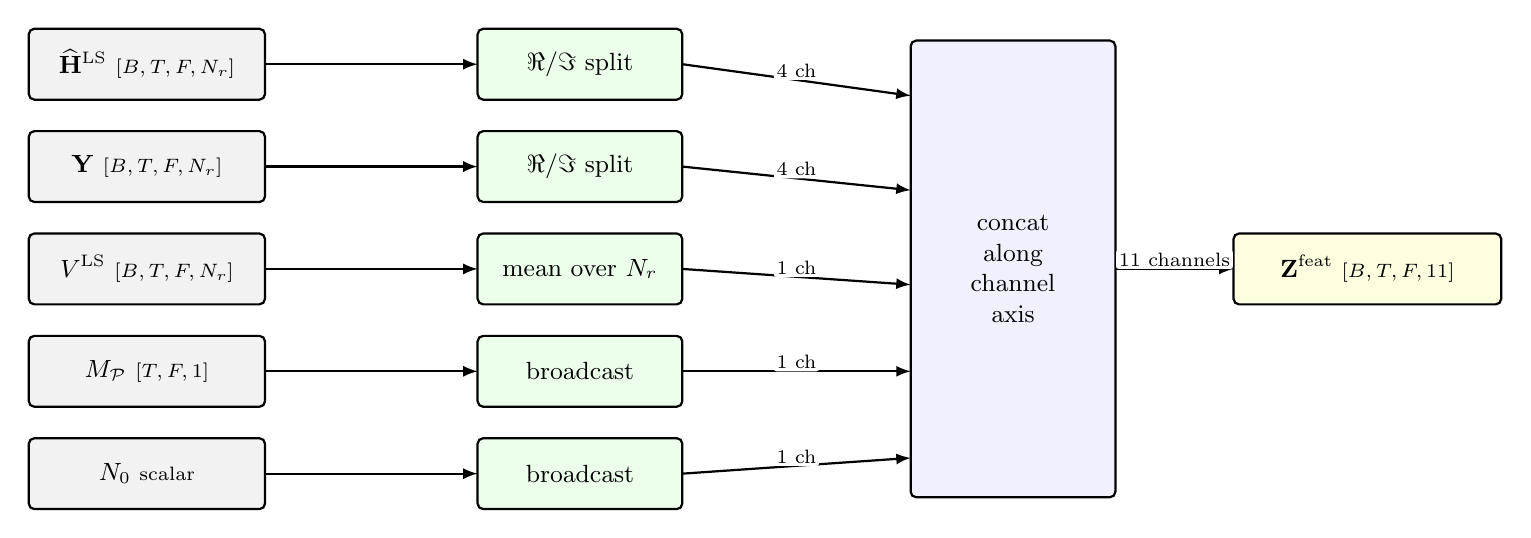
\begin{tikzpicture}[x=1cm, y=1cm, >=latex]
				\node[io, minimum width=3.0cm, minimum height=0.9cm] at (0.00,2.40) (hls) {$\widehat{\mathbf{H}}^{\mathrm{LS}}$ \scriptsize{$[B,T,F,N_r]$}};
				\node[io, minimum width=3.0cm, minimum height=0.9cm] at (0.00,1.10) (y) {$\mathbf{Y}$ \scriptsize{$[B,T,F,N_r]$}};
				\node[io, minimum width=3.0cm, minimum height=0.9cm] at (0.00,-0.20) (vls) {$V^{\mathrm{LS}}$ \scriptsize{$[B,T,F,N_r]$}};
				\node[io, minimum width=3.0cm, minimum height=0.9cm] at (0.00,-1.50) (mp) {$M_{\mathcal{P}}$ \scriptsize{$[T,F,1]$}};
				\node[io, minimum width=3.0cm, minimum height=0.9cm] at (0.00,-2.80) (n0) {$N_0$ \scriptsize{scalar}};
				\node[op, minimum width=2.6cm, minimum height=0.9cm] at (5.50,2.40) (ri1) {$\Re/\Im$ split};
				\node[op, minimum width=2.6cm, minimum height=0.9cm] at (5.50,1.10) (ri2) {$\Re/\Im$ split};
				\node[op, minimum width=2.6cm, minimum height=0.9cm] at (5.50,-0.20) (avg) {mean over $N_r$};
				\node[op, minimum width=2.6cm, minimum height=0.9cm] at (5.50,-1.50) (bc1) {broadcast};
				\node[op, minimum width=2.6cm, minimum height=0.9cm] at (5.50,-2.80) (bc2) {broadcast};
				\node[dat, minimum width=2.6cm, minimum height=5.8cm] at (11.00,-0.20) (cat) {concat\\along\\channel\\axis};
				\node[outp, minimum width=3.4cm, minimum height=0.9cm] at (15.50,-0.20) (out1) {$\mathbf{Z}^{\mathrm{feat}}$ \scriptsize{$[B,T,F,11]$}};
				\draw[thick, ->] (1.50,2.40) -- (4.20,2.40);
				\draw[thick, ->] (1.50,1.10) -- (4.20,1.10);
				\draw[thick, ->] (1.50,-0.20) -- (4.20,-0.20);
				\draw[thick, ->] (1.50,-1.50) -- (4.20,-1.50);
				\draw[thick, ->] (1.50,-2.80) -- (4.20,-2.80);
				\draw[thick, ->] (6.80,2.40) -- (9.70,2.00) node[lbl, pos=0.5, above] {4 ch};
				\draw[thick, ->] (6.80,1.10) -- (9.70,0.80) node[lbl, pos=0.5, above] {4 ch};
				\draw[thick, ->] (6.80,-0.20) -- (9.70,-0.40) node[lbl, pos=0.5, above] {1 ch};
				\draw[thick, ->] (6.80,-1.50) -- (9.70,-1.50) node[lbl, pos=0.5, above] {1 ch};
				\draw[thick, ->] (6.80,-2.80) -- (9.70,-2.60) node[lbl, pos=0.5, above] {1 ch};
				\draw[thick, ->] (12.30,-0.20) -- (13.80,-0.20) node[lbl, pos=0.5, above] {11 channels};
			\end{tikzpicture}%
		}
		\caption{Section~4.2: Input feature tensor assembly.  Five inputs produce 11 real-valued channels.}
		\label{fig:sec42}
	\end{figure}
	
	\subsection{The 1$\times$1 Stem Convolution}
	
	A $1 \times 1$ convolution has a kernel of spatial size one: it looks at exactly \emph{one} grid position at a time, with no spatial neighbours involved.  Unlike a standard $3 \times 3$ convolution that mixes information from a local patch, a $1 \times 1$ convolution performs purely \textbf{channel mixing}: at each position independently, it takes the vector of input channels and maps it to a new vector of output channels through a learned linear transformation.
	
	Concretely, at each time--frequency position $(t,f)$ the 11-dimensional input feature vector $\bZ^{\mathrm{feat}}_{b,t,f,:} \in \mathbb{R}^{11}$ is mapped to a 96-dimensional hidden vector by:
	\begin{equation}
		\bZ^{(0)}_{b,t,f,:} = W_{\mathrm{stem}}\,\bZ^{\mathrm{feat}}_{b,t,f,:} + \mathbf{b}_{\mathrm{stem}},
		\label{eq:stem}
	\end{equation}
	where $W_{\mathrm{stem}} \in \mathbb{R}^{96 \times 11}$ and $\mathbf{b}_{\mathrm{stem}} \in \mathbb{R}^{96}$ are learned parameters.  The \emph{same} $W_{\mathrm{stem}}$ and $\mathbf{b}_{\mathrm{stem}}$ are applied at every position on the grid---the operation is translation-invariant, just like any convolution.
	
	Each of the 96 rows of $W_{\mathrm{stem}}$ defines one output channel as a weighted combination of the 11 input features.  After training, these rows learn to compute whatever linear combinations of the raw inputs are most useful for the downstream processing---for example, differences between the LS estimate and the raw received signal, channel magnitude features, or combinations that weight the noise and pilot-mask features differently depending on position type.
	
	The stem is intentionally $1 \times 1$ rather than $3 \times 3$ because its job is not to detect spatial patterns.  The spatial relationships between neighbouring subcarriers and symbols are handled later by the attention layers and the depthwise convolution.  Using a larger kernel here would mix spatial neighbours before the network has had a chance to process the per-position features, potentially blurring important local structure---such as the sharp boundary between a pilot position ($M_{\mathcal{P}} = 1$, reliable LS estimate) and an adjacent data position ($M_{\mathcal{P}} = 0$, interpolated LS estimate).
	
	The term ``stem'' comes from the vision transformer literature, where raw input features are projected into a higher-dimensional working space before the transformer layers.  Here, the stem is the transition from the 11-dimensional physical feature domain to the 96-dimensional learned representation in which all subsequent processing---prompt computation, FiLM modulation, axial attention, output heads---takes place.
	
	
	
	\begin{figure}[ht!]
		\centering
		\resizebox{0.72\linewidth}{!}{%
			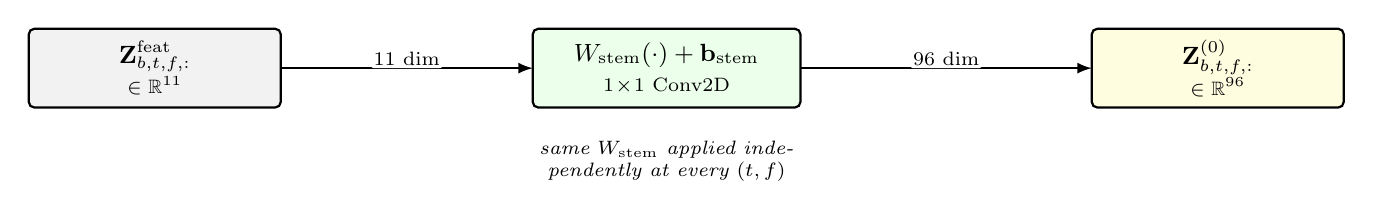
\begin{tikzpicture}[x=1cm, y=1cm, >=latex]
				\node[io, minimum width=3.2cm, minimum height=1.0cm] at (0.00,0.00) (inp) {$\mathbf{Z}^{\mathrm{feat}}_{b,t,f,:}$\\{\scriptsize $\in\mathbb{R}^{11}$}};
				\node[op, minimum width=3.4cm, minimum height=1.0cm] at (6.50,0.00) (stem) {$W_{\mathrm{stem}}(\cdot)+\mathbf{b}_{\mathrm{stem}}$\\{\scriptsize $1\!\times\!1$ Conv2D}};
				\node[outp, minimum width=3.2cm, minimum height=1.0cm] at (13.50,0.00) (out1) {$\mathbf{Z}^{(0)}_{b,t,f,:}$\\{\scriptsize $\in\mathbb{R}^{96}$}};
				\draw[thick, ->] (1.60,0.00) -- (4.80,0.00) node[lbl, pos=0.5, above] {11 dim};
				\draw[thick, ->] (8.20,0.00) -- (11.90,0.00) node[lbl, pos=0.5, above] {96 dim};
				\node[font=\scriptsize\itshape, anchor=north, text width=6cm, align=center] at (6.50,-0.80) {same $W_{\mathrm{stem}}$ applied independently at every $(t,f)$};
			\end{tikzpicture}%
		}
		\caption{Section~4.3: $1\!\times\!1$ stem convolution.  Per-position projection from 11 to 96 channels.}
		\label{fig:sec43}
	\end{figure}
	
	\subsection{The Pilot-Conditioned Prompt}
	\label{sec:prompt}
	
	After the stem produces $\bZ^{(0)} \in \mathbb{R}^{B \times T \times F \times 96}$, the network computes a single conditioning vector per slot---the \emph{prompt}---that will later modulate every layer through FiLM.  The computation has three stages, each with a clear purpose.
	
	\medskip\noindent
	\textbf{Stage 1: Pilot masking.}\quad
	The stem output is multiplied element-wise by the pilot mask, zeroing out all data positions:
	\begin{equation}
		\widetilde{\bZ}^{(0)}_{b,t,f,:} = M_\mathcal{P}[t,f] \cdot \bZ^{(0)}_{b,t,f,:}.
		\label{eq:prompt_mask}
	\end{equation}
	At pilot positions ($M_\mathcal{P} = 1$), the stem features pass through unchanged.  At data positions ($M_\mathcal{P} = 0$), they become zero.  This is a hard gate, not a soft weighting.
	
	\medskip\noindent
	\textbf{Stage 2: Spatial average pooling.}\quad
	The masked features are summed over the entire time--frequency grid and divided by the number of pilot positions:
	\begin{equation}
		\bar{\bZ}_b = \frac{\displaystyle\sum_{t=0}^{T-1}\sum_{f=0}^{F-1} \widetilde{\bZ}^{(0)}_{b,t,f,:}}{\displaystyle\sum_{t=0}^{T-1}\sum_{f=0}^{F-1} M_\mathcal{P}[t,f] + 10^{-6}} \;\in\; \mathbb{R}^{96}.
		\label{eq:prompt_pool}
	\end{equation}
	Because $\widetilde{\bZ}^{(0)}$ is zero at data positions, only pilot positions contribute to the numerator.  The result $\bar{\bZ}_b$ is a single 96-dimensional vector that represents the \emph{average pilot-region representation} for batch element $b$.  Different slots produce different $\bar{\bZ}_b$ because the channel, noise, and phase conditions at the pilot positions are different.
	
	\medskip\noindent
	\textbf{Stage 3: Prompt MLP.}\quad
	The pooled vector is passed through a two-layer multilayer perceptron to produce the final prompt:
	\begin{align}
		\bh_b &= \GELU\!\left(W_1\,\bar{\bZ}_b + \mathbf{b}_1\right), \label{eq:prompt_mlp1} \\
		\bp_b &= W_2\,\bh_b + \mathbf{b}_2, \label{eq:prompt_mlp2}
	\end{align}
	where $W_1 \in \mathbb{R}^{96 \times 96}$, $\mathbf{b}_1 \in \mathbb{R}^{96}$, $W_2 \in \mathbb{R}^{96 \times 96}$, and $\mathbf{b}_2 \in \mathbb{R}^{96}$.  The first layer applies a linear transformation followed by a GELU nonlinearity.  The second layer is a purely linear projection with no activation.
	
	\begin{warning}
		The nonlinearity between the two layers is essential.  Without it, the composition $W_2(W_1 \bar{\bZ}_b + \mathbf{b}_1) + \mathbf{b}_2$ collapses to a single linear transformation $W'\bar{\bZ}_b + \mathbf{b}'$, which would limit the prompt to linear functions of the pooled features.  The GELU activation allows the prompt MLP to compute nonlinear summaries---for instance, it can learn to respond differently to high-SNR versus low-SNR pilot regions, or to detect the presence of a deep fade at the DMRS symbol.
	\end{warning}
	
	The final prompt $\bp_b \in \mathbb{R}^{96}$ is a compact, nonlinear summary of the current slot's pilot-region characteristics.  It encodes answers to questions like: ``How noisy is this slot?'', ``How frequency-selective is the channel at the DMRS?'', ``How strong is the signal at the pilot positions?''  Importantly, $\bp_b$ is \emph{not} a learnable free parameter---it is a deterministic function of the current slot's received signal.  The same weights $(W_1, \mathbf{b}_1, W_2, \mathbf{b}_2)$ are applied to every slot, but different slot conditions produce different prompts, which in turn produce different FiLM modulations in every downstream layer.
	
	
	
	\begin{figure}[ht!]
		\centering
		\resizebox{1\linewidth}{!}{%
			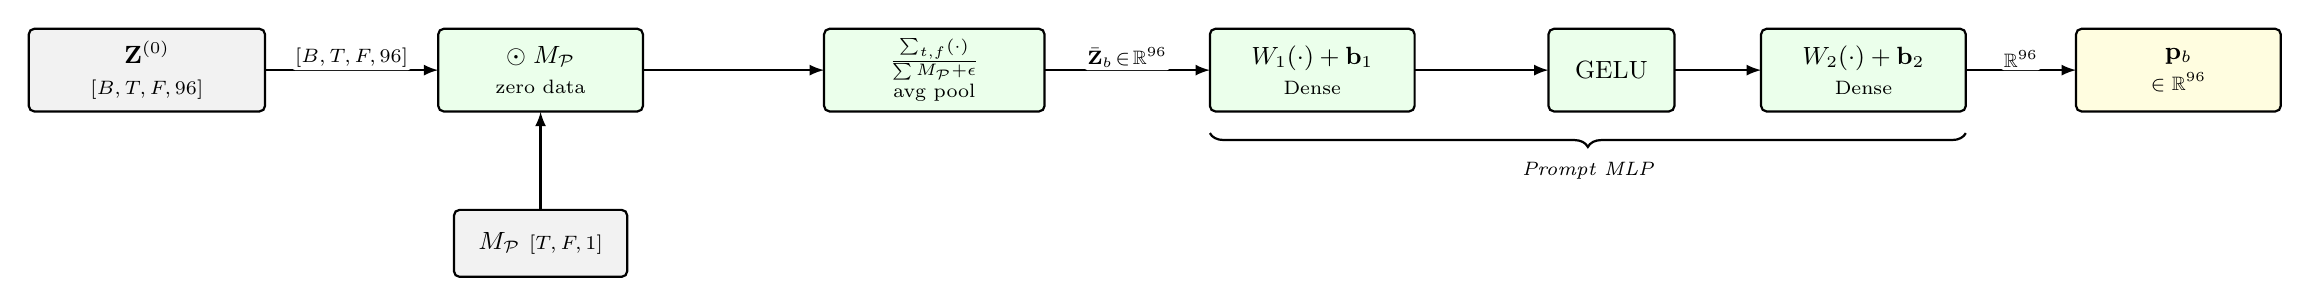
\begin{tikzpicture}[x=1cm, y=1cm, >=latex]
				\node[io, minimum width=3.0cm, minimum height=1.05cm] at (0.00,0.00) (z0) {$\mathbf{Z}^{(0)}$\\{\scriptsize $[B,T,F,96]$}};
				\node[op, minimum width=2.6cm, minimum height=1.05cm] at (5.00,0.00) (mask) {$\odot\;M_{\mathcal{P}}$\\{\scriptsize zero data}};
				\node[op, minimum width=2.8cm, minimum height=1.05cm] at (10.00,0.00) (pool) {$\frac{\sum_{t,f}(\cdot)}{\sum M_{\mathcal{P}}+\epsilon}$\\{\scriptsize avg pool}};
				\node[op, minimum width=2.6cm, minimum height=1.05cm] at (14.80,0.00) (fc1) {$W_1(\cdot)+\mathbf{b}_1$\\{\scriptsize Dense}};
				\node[op, minimum width=1.6cm, minimum height=1.05cm] at (18.60,0.00) (gelu) {GELU};
				\node[op, minimum width=2.6cm, minimum height=1.05cm] at (21.80,0.00) (fc2) {$W_2(\cdot)+\mathbf{b}_2$\\{\scriptsize Dense}};
				\node[outp, minimum width=2.6cm, minimum height=1.05cm] at (25.80,0.00) (out1) {$\mathbf{p}_b$\\{\scriptsize $\in\mathbb{R}^{96}$}};
				\node[io, minimum width=2.2cm, minimum height=0.85cm] at (5.00,-2.20) (mp) {$M_{\mathcal{P}}$ \scriptsize{$[T,F,1]$}};
				\draw[thick, ->] (1.50,0.00) -- (3.70,0.00) node[lbl, pos=0.5, above] {$[B,T,F,96]$};
				\draw[thick, ->] (5.00,-1.78) -- (5.00,-0.53);
				\draw[thick, ->] (6.30,0.00) -- (8.60,0.00);
				\draw[thick, ->] (11.40,0.00) -- (13.50,0.00) node[lbl, pos=0.5, above] {$\bar{\mathbf{Z}}_b\!\in\!\mathbb{R}^{96}$};
				\draw[thick, ->] (16.10,0.00) -- (17.80,0.00);
				\draw[thick, ->] (19.40,0.00) -- (20.50,0.00);
				\draw[thick, ->] (23.10,0.00) -- (24.50,0.00) node[lbl, pos=0.5, above] {$\mathbb{R}^{96}$};
				\draw[decorate, decoration={brace, mirror, amplitude=5pt}, thick] (13.50,-0.80) -- (23.10,-0.80) node[midway, below=7pt, font=\scriptsize\itshape] {Prompt MLP};
			\end{tikzpicture}%
		}
		\caption{Section~4.4: Pilot-conditioned prompt.  Masked pooling then two-layer MLP.}
		\label{fig:sec44}
	\end{figure}
	
	\subsection{Feature-wise Linear Modulation (FiLM)}
	\label{sec:film}
	
	FiLM was introduced by Perez et al.\ (2018) for visual question answering and has since become a standard conditioning mechanism.  The idea is to let an external signal control a neural network's internal representations through learned scaling and shifting.
	
	Given a hidden feature tensor $\mathbf{u} \in \mathbb{R}^{B \times T \times F \times d}$ and a conditioning vector $\bp \in \mathbb{R}^{B \times d}$, FiLM computes:
	\begin{equation}
		\FiLM(\mathbf{u}, \bp) = \mathbf{u} \odot (1 + \boldsymbol{\gamma}) + \boldsymbol{\beta},
		\label{eq:film}
	\end{equation}
	where $\boldsymbol{\gamma}, \boldsymbol{\beta} \in \mathbb{R}^{B \times d}$ are computed from the prompt:
	\begin{equation}
		[\boldsymbol{\gamma}, \boldsymbol{\beta}] = W_{\mathrm{FiLM}}\, \bp + \mathbf{b}_{\mathrm{FiLM}}.
	\end{equation}
	
	The key properties:
	\begin{itemize}[nosep]
		\item $\boldsymbol{\gamma}$ and $\boldsymbol{\beta}$ are \emph{vectors} with the same dimension as the feature channels (96).
		\item They are \emph{broadcast} across all spatial positions $(t,f)$.  Every position gets the same modulation---but the modulation depends on the current slot's prompt.
		\item $\boldsymbol{\gamma}$ provides multiplicative scaling (can amplify or suppress channels).
		\item $\boldsymbol{\beta}$ provides additive shifting (can bias channels).
		\item The cost is negligible: one linear projection of a 96-dimensional vector.
	\end{itemize}
	
	\textbf{Why FiLM and not alternatives?}
	\begin{itemize}[nosep]
		\item \emph{Concatenation} (appending $\bp$ to every position) increases the dimension and makes every layer larger.
		\item \emph{Addition only} (just adding $\bp$) can shift but not scale.
		\item \emph{Cross-attention} (letting features attend to $\bp$) is powerful but expensive.
		\item \emph{FiLM} is cheap, expressive (both scaling and shifting), and doesn't change tensor dimensions.
	\end{itemize}
	
	In UPAIR-5G, FiLM is used in a \textbf{normalise-then-modulate} pattern: LayerNorm first normalises the features, then FiLM rescales them based on the slot context.  This combination is numerically stable and effective.
	
	\begin{keyidea}
		FiLM is the mechanism by which the prompt controls the network.  Different slots produce different $\boldsymbol{\gamma}, \boldsymbol{\beta}$, which produce different internal representations, which produce different channel corrections---all in one forward pass.
	\end{keyidea}
	
	
	
	\begin{figure}[ht!]
		\centering
		\resizebox{1\linewidth}{!}{%
			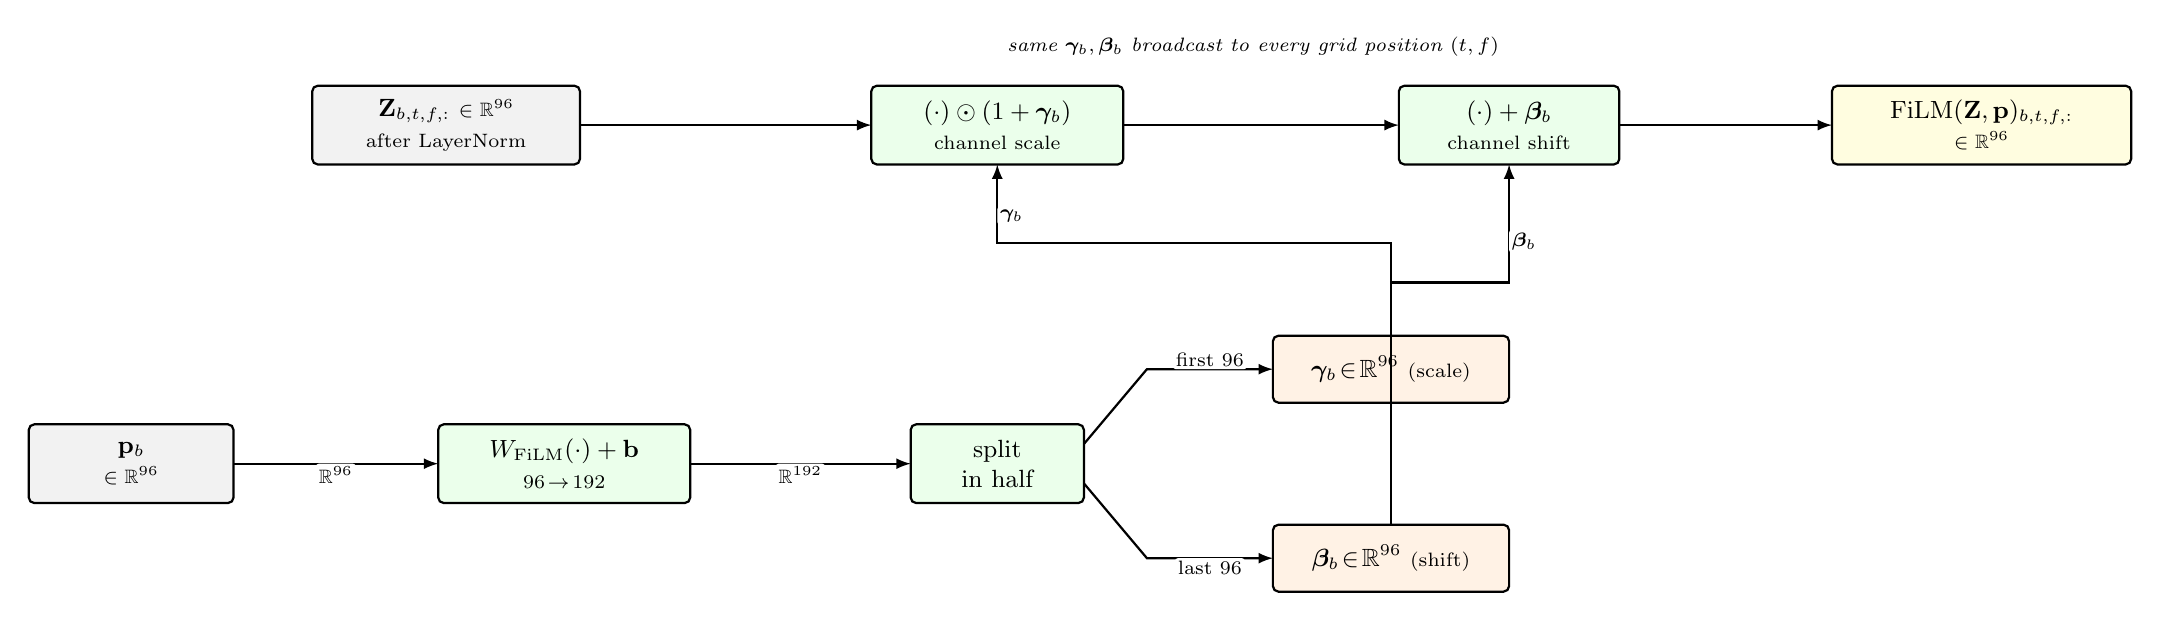
\begin{tikzpicture}[x=1cm, y=1cm, >=latex]
				\node[io, minimum width=2.6cm, minimum height=1.0cm] at (0.00,-2.50) (pr) {$\mathbf{p}_b$\\{\scriptsize $\in\mathbb{R}^{96}$}};
				\node[op, minimum width=3.2cm, minimum height=1.0cm] at (5.50,-2.50) (proj) {$W_{\mathrm{FiLM}}(\cdot)+\mathbf{b}$\\{\scriptsize $96\!\to\!192$}};
				\node[op, minimum width=2.2cm, minimum height=1.0cm] at (11.00,-2.50) (spl) {split\\in half};
				\node[aux, minimum width=3.0cm, minimum height=0.85cm] at (16.00,-1.30) (gam) {$\boldsymbol{\gamma}_b\!\in\!\mathbb{R}^{96}$ {\scriptsize (scale)}};
				\node[aux, minimum width=3.0cm, minimum height=0.85cm] at (16.00,-3.70) (bet) {$\boldsymbol{\beta}_b\!\in\!\mathbb{R}^{96}$ {\scriptsize (shift)}};
				\node[io, minimum width=3.4cm, minimum height=1.0cm] at (4.00,1.80) (zin) {$\mathbf{Z}_{b,t,f,:}$ \scriptsize{$\in\mathbb{R}^{96}$}\\{\scriptsize after LayerNorm}};
				\node[op, minimum width=3.2cm, minimum height=1.0cm] at (11.00,1.80) (mul) {$(\cdot)\odot(1+\boldsymbol{\gamma}_b)$\\{\scriptsize channel scale}};
				\node[op, minimum width=2.8cm, minimum height=1.0cm] at (17.50,1.80) (add) {$(\cdot)+\boldsymbol{\beta}_b$\\{\scriptsize channel shift}};
				\node[outp, minimum width=3.8cm, minimum height=1.0cm] at (23.50,1.80) (zout) {$\mathrm{FiLM}(\mathbf{Z},\mathbf{p})_{b,t,f,:}$\\{\scriptsize $\in\mathbb{R}^{96}$}};
				\draw[thick, ->] (1.30,-2.50) -- (3.90,-2.50) node[lbl, pos=0.5, below] {$\mathbb{R}^{96}$};
				\draw[thick, ->] (7.10,-2.50) -- (9.90,-2.50) node[lbl, pos=0.5, below] {$\mathbb{R}^{192}$};
				\draw[thick, ->] (12.10,-2.25) -- (12.90,-1.30) -- (14.50,-1.30) node[lbl, pos=0.5, above] {first 96};
				\draw[thick, ->] (12.10,-2.75) -- (12.90,-3.70) -- (14.50,-3.70) node[lbl, pos=0.5, below] {last 96};
				\draw[thick, ->] (5.70,1.80) -- (9.40,1.80);
				\draw[thick, ->] (16.00,-0.88) -- (16.00,0.30) -- (11.00,0.30) -- (11.00,1.30) node[lbl, pos=0.35, right] {$\boldsymbol{\gamma}_b$};
				\draw[thick, ->] (12.60,1.80) -- (16.10,1.80);
				\draw[thick, ->] (16.00,-3.28) -- (16.00,-0.20) -- (17.50,-0.20) -- (17.50,1.30) node[lbl, pos=0.35, right] {$\boldsymbol{\beta}_b$};
				\draw[thick, ->] (18.90,1.80) -- (21.60,1.80);
				\node[font=\scriptsize\itshape, anchor=south, text width=8cm, align=center] at (14.25,2.55) {same $\boldsymbol{\gamma}_b,\boldsymbol{\beta}_b$ broadcast to every grid position $(t,f)$};
			\end{tikzpicture}%
		}
		\caption{Section~4.5: FiLM.  Prompt produces per-channel scale ($\boldsymbol{\gamma}$) and shift ($\boldsymbol{\beta}$), applied at every position.}
		\label{fig:sec45}
	\end{figure}
	
	\subsection{Axial Attention}
	
	\subsubsection*{The problem attention solves}
	
	After the stem and FiLM, the network has a tensor $\mathbf{Z}$ of shape $[B, T, F, 96]$---a 96-dimensional feature vector at every point on the time--frequency grid.  Right now, each grid position only knows about \emph{itself}.  But the channel at position $(t\!=\!5, f\!=\!100)$ is correlated with the channel at $(t\!=\!5, f\!=\!101)$ (nearby subcarriers experience similar multipath) and with $(t\!=\!6, f\!=\!100)$ (the channel evolves smoothly in time).  To perform good interpolation, the network needs to let grid positions \textbf{share information} with each other.  Attention is the mechanism for this: each position computes a weighted combination of all other positions' features, where the weights are learned based on how relevant each pair is.
	
	\subsubsection*{The axial factorisation idea}
	
	Instead of one massive 2D attention (every grid position attending to every other), axial attention breaks it into two cheap 1D attentions applied \emph{sequentially}.  Think of it like this: if you need to go from corner~A to corner~C of a rectangular room, you do not need to search the whole floor---you can walk along one wall (handle one axis), then along the other wall (handle the other axis).  Information still propagates everywhere, just in two hops instead of one.
	
	\subsubsection*{How single-head attention works}
	
	Before describing the two stages, we need the attention equations.  Suppose we have a sequence of $N$ positions, each carrying a $d$-dimensional feature vector, arranged as a matrix $\mathbf{U} \in \mathbb{R}^{N \times d}$.  (In frequency attention, $N\!=\!F\!=\!192$ and the positions are subcarriers; in time attention, $N\!=\!T\!=\!14$ and the positions are OFDM symbols.)
	
	Each position is projected into three roles through learned weight matrices:
	\begin{align}
		\mathbf{Q} &= \mathbf{U}\,W_Q, \qquad W_Q \in \mathbb{R}^{d \times d_k}, \label{eq:attn_q}\\
		\mathbf{K} &= \mathbf{U}\,W_K, \qquad W_K \in \mathbb{R}^{d \times d_k}, \label{eq:attn_k}\\
		\mathbf{V} &= \mathbf{U}\,W_V, \qquad W_V \in \mathbb{R}^{d \times d_v}, \label{eq:attn_v}
	\end{align}
	where $\mathbf{Q}$ is the \textbf{query} (``what am I looking for?''), $\mathbf{K}$ is the \textbf{key} (``what do I contain?''), and $\mathbf{V}$ is the \textbf{value} (``what information do I provide if selected?'').  The query and key have dimension $d_k$; the value has dimension $d_v$.
	
	The attention output is:
	\begin{equation}
		\mathrm{Attention}(\mathbf{Q}, \mathbf{K}, \mathbf{V}) = \underbrace{\mathrm{softmax}\!\left(\frac{\mathbf{Q}\,\mathbf{K}^T}{\sqrt{d_k}}\right)}_{\displaystyle\mathbf{A}\;\in\;\mathbb{R}^{N \times N}} \;\mathbf{V}.
		\label{eq:attn_sdp}
	\end{equation}
	
	The matrix product $\mathbf{Q}\,\mathbf{K}^T \in \mathbb{R}^{N \times N}$ computes a \emph{relevance score} between every pair of positions: entry $(i,j)$ measures how much position~$i$'s query matches position~$j$'s key.  Dividing by $\sqrt{d_k}$ prevents the scores from becoming too large (which would push the softmax into saturation).  The row-wise softmax converts scores into non-negative weights that sum to one---these are the \textbf{attention weights} $\mathbf{A}$.  Finally, multiplying by $\mathbf{V}$ produces the output: each position's new representation is a weighted average of all positions' values, where the weights reflect relevance.
	
	\begin{warning}
		The key insight: attention is a \emph{data-dependent} weighted average.  Unlike a fixed filter (e.g., a convolution kernel), the weights change depending on the actual content at each position.  If subcarrier~$f\!=\!50$ happens to have a channel feature similar to $f\!=\!120$ in a particular slot, attention will assign a high weight between them---even though they are far apart.  A fixed filter cannot do this.
	\end{warning}
	
	\subsubsection*{Multi-head attention}
	
	A single set of $(W_Q, W_K, W_V)$ can only capture one notion of ``relevance.''  Multi-head attention runs $H$ independent attention operations in parallel, each with its own projections, and concatenates the results:
	\begin{align}
		\mathrm{head}_h &= \mathrm{Attention}\!\left(\mathbf{U}\,W_Q^{(h)},\; \mathbf{U}\,W_K^{(h)},\; \mathbf{U}\,W_V^{(h)}\right), \qquad h = 1,\dots,H, \label{eq:mha_head}\\
		\mathrm{MHA}(\mathbf{U}) &= \Concat\!\left(\mathrm{head}_1,\;\dots,\;\mathrm{head}_H\right) W_O, \label{eq:mha_concat}
	\end{align}
	where each head operates on dimension $d_k = d_v = d/H$, and $W_O \in \mathbb{R}^{d \times d}$ is a final output projection that mixes the heads back together.
	
	In UPAIR-5G, $d\!=\!96$ and $H\!=\!4$, so each head works with $d_k\!=\!d_v\!=\!24$ dimensions.  Different heads can learn different aspects of the correlation structure---for example, one head might focus on short-range frequency correlations (nearby subcarriers), another on long-range patterns, and a third on the relationship between pilot and data positions.
	
	\subsubsection*{Stage~1---Frequency attention (top row of Fig.~\ref{fig:sec46})}
	
	The goal is: within each OFDM symbol, let subcarriers share information with each other.  This captures \textbf{frequency-domain structure}---the multipath delay profile creates correlations across subcarriers.  Follow the top row of the diagram left to right:
	
	\begin{enumerate}[nosep]
		\item $\mathbf{Z}$ $[B, T, F, 96]$ enters from the left.  This is a 4D tensor: $B$~batch elements, $T\!=\!14$ OFDM symbols, $F\!=\!192$ subcarriers, $96$~feature channels.
		
		\item \textbf{Reshape to $[\,B \!\cdot\! T,\; F,\; 96\,]$.}  This is a pure bookkeeping operation---no computation, no learned parameters.  It ``stacks'' the batch and time dimensions together.  The result is $B \!\cdot\! T$ independent sequences, each of length $F\!=\!192$, each with 96~features.  The attention mechanism treats each of the $B \!\cdot\! T$ sequences independently.  \emph{Why?}  Because we want frequency attention to operate \emph{within a single OFDM symbol}.  By merging $B$ and $T$, each OFDM symbol becomes its own independent ``sentence'' of length~192, and the attention will let the 192 ``tokens'' (subcarriers) attend to each other.
		
		\item \textbf{Multi-Head Attn (freq).}  For each of the $B \!\cdot\! T$ sequences, apply equations~\eqref{eq:attn_q}--\eqref{eq:mha_concat} with $N\!=\!F\!=\!192$ and $\mathbf{U} \in \mathbb{R}^{192 \times 96}$.  Each of the 192 subcarrier positions produces a query, key, and value vector.  The attention weights tell subcarrier~$f$ ``how much to listen to'' every other subcarrier~$f'$.  The network might learn, for example, that nearby subcarriers are highly relevant (short delay spread $\to$ smooth channel), or that periodic subcarrier patterns matter (delay spread creates a sinc-like correlation in frequency).
		
		\item \textbf{Reshape back to $[B, T, F, 96]$.}  Un-stack the batch and time dimensions.  The tensor is back to its original shape, but now each position's 96-dimensional feature vector has been enriched with information from all other subcarriers within the same OFDM symbol.
	\end{enumerate}
	
	\subsubsection*{The diagonal arrow: connecting the two stages}
	
	In the diagram, the output of frequency attention (after the reshape back) goes diagonally down-left into the ``transpose'' box of time attention.  This arrow represents the sequential composition: the frequency-enriched features enter time attention next.  Note that \emph{no arrow goes from frequency attention directly to the output $\mathbf{Z}'$}---the only path to $\mathbf{Z}'$ is through time attention.
	
	\subsubsection*{Stage~2---Time attention (bottom row of Fig.~\ref{fig:sec46})}
	
	The goal now flips: within each subcarrier, let OFDM symbols share information across time.  This captures \textbf{time-domain structure}---Doppler shifts and phase drift create correlations across OFDM symbols.
	
	\begin{enumerate}[nosep]
		\item \textbf{Transpose to $[B, F, T, 96]$.}  Swap the $T$ and $F$ axes.  Now $F$ is in the ``batch-like'' position and $T$ is in the ``sequence'' position.
		
		\item \textbf{Reshape to $[\,B \!\cdot\! F,\; T,\; 96\,]$.}  Same trick as before, but now merging batch and frequency.  The result is $B \!\cdot\! F$ independent sequences, each of length $T\!=\!14$.  Each subcarrier becomes its own ``sentence'' of 14 ``tokens'' (OFDM symbols).
		
		\item \textbf{Multi-Head Attn (time).}  Apply equations~\eqref{eq:attn_q}--\eqref{eq:mha_concat} with $N\!=\!T\!=\!14$ and $\mathbf{U} \in \mathbb{R}^{14 \times 96}$.  Self-attention runs across the 14 time positions.  Each OFDM symbol can attend to every other symbol.  The network might learn that symbols close in time are more relevant (slow fading), or that the DMRS symbol ($t\!=\!2$) is especially important (it is where the reliable pilot observations are).  This is also where the network can implicitly learn to track phase drift---by comparing features across symbols, attention can detect systematic phase rotation.
		
		\item \textbf{Reshape + transpose back.}  Un-stack and un-transpose to recover $[B, T, F, 96]$.  The upward arrow in the diagram shows this result feeding back up to become the final output $\mathbf{Z}'$.
	\end{enumerate}
	
	\subsubsection*{What has been achieved after both stages?}
	
	After Stage~1, each position knows about its frequency neighbours (within the same OFDM symbol).  After Stage~2, each position knows about its time neighbours (within the same subcarrier).  But crucially, through the sequential composition, information can also propagate \textbf{diagonally} across the grid: position $(t\!=\!2, f\!=\!50)$ can send information to $(t\!=\!2, f\!=\!100)$ during frequency attention, and then $(t\!=\!2, f\!=\!100)$ can forward that information to $(t\!=\!8, f\!=\!100)$ during time attention.  So $(t\!=\!8, f\!=\!100)$ has indirectly received information from $(t\!=\!2, f\!=\!50)$---a position it never directly attended to.  Two hops cover the entire grid.
	
	\begin{keyidea}
		Imagine filling in a crossword puzzle where the ``clues'' are only at certain squares (the pilot positions).  Frequency attention is like solving each \emph{row}---using known letters in that row to constrain unknown ones.  Time attention is like solving each \emph{column}---using known letters in that column to constrain unknown ones.  You never solve the full 2D grid simultaneously, but by alternating row-solves and column-solves, information propagates everywhere.  This is exactly what axial attention does: alternate between ``solve along frequency'' and ``solve along time.''
	\end{keyidea}
	
	
	
	\begin{figure}[ht!]
		\centering
		\resizebox{1\linewidth}{!}{%
			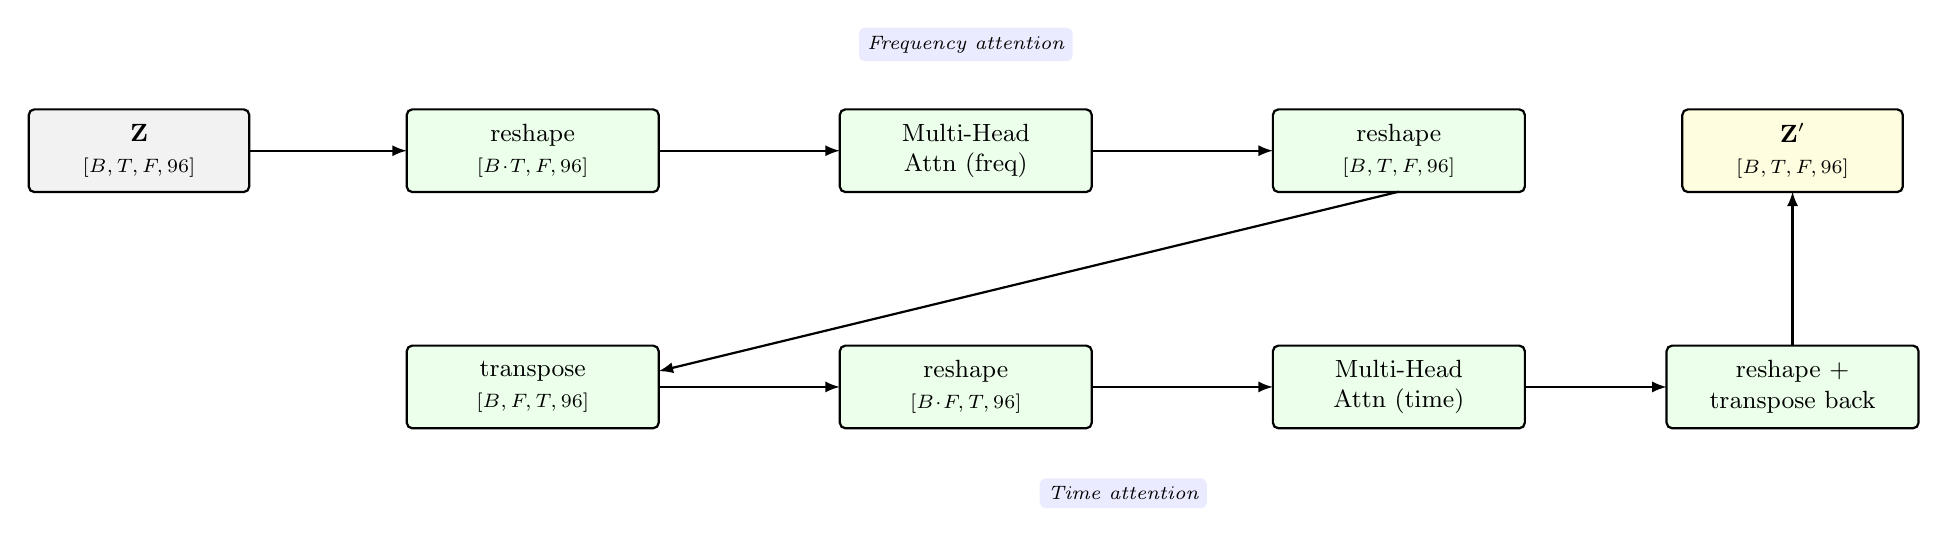
\begin{tikzpicture}[x=1cm, y=1cm, >=latex]
				\node[io, minimum width=2.8cm, minimum height=1.05cm] at (0.00,2.20) (zin) {$\mathbf{Z}$\\{\scriptsize $[B,T,F,96]$}};
				\node[op, minimum width=3.2cm, minimum height=1.05cm] at (5.00,2.20) (r1) {reshape\\{\scriptsize $[B\!\cdot\! T,F,96]$}};
				\node[op, minimum width=3.2cm, minimum height=1.05cm] at (10.50,2.20) (mhaf) {Multi-Head\\Attn (freq)};
				\node[op, minimum width=3.2cm, minimum height=1.05cm] at (16.00,2.20) (r2) {reshape\\{\scriptsize $[B,T,F,96]$}};
				\node[outp, minimum width=2.8cm, minimum height=1.05cm] at (21.00,2.20) (zout) {$\mathbf{Z}'$\\{\scriptsize $[B,T,F,96]$}};
				\node[op, minimum width=3.2cm, minimum height=1.05cm] at (5.00,-0.80) (tr) {transpose\\{\scriptsize $[B,F,T,96]$}};
				\node[op, minimum width=3.2cm, minimum height=1.05cm] at (10.50,-0.80) (r3) {reshape\\{\scriptsize $[B\!\cdot\! F,T,96]$}};
				\node[op, minimum width=3.2cm, minimum height=1.05cm] at (16.00,-0.80) (mhat) {Multi-Head\\Attn (time)};
				\node[op, minimum width=3.2cm, minimum height=1.05cm] at (21.00,-0.80) (r4) {reshape +\\transpose back};
				\draw[thick, ->] (1.40,2.20) -- (3.40,2.20);
				\draw[thick, ->] (6.60,2.20) -- (8.90,2.20);
				\draw[thick, ->] (12.10,2.20) -- (14.40,2.20);
				\draw[thick, ->] (16.00,1.68) -- (6.60,-0.60);
				\draw[thick, ->] (6.60,-0.80) -- (8.90,-0.80);
				\draw[thick, ->] (12.10,-0.80) -- (14.40,-0.80);
				\draw[thick, ->] (17.60,-0.80) -- (19.40,-0.80);
				\draw[thick, ->] (21.00,-0.28) -- (21.00,1.68);
				\node[font=\scriptsize\itshape, fill=blue!8, rounded corners=2pt, inner sep=3pt] at (10.50,3.55) {Frequency attention};
				\node[font=\scriptsize\itshape, fill=blue!8, rounded corners=2pt, inner sep=3pt] at (12.50,-2.15) {Time attention};
			\end{tikzpicture}%
		}
		\caption{Section~4.6: Internal reshaping mechanics of axial attention.  Frequency (top) then time (bottom).}
		\label{fig:sec46}
	\end{figure}
	
	\begin{warning}
		This figure shows only the \emph{internal reshaping mechanics} of the attention operations---what happens inside the ``Freq MHA'' and ``Time MHA'' boxes.  In the actual architecture (Fig.~\ref{fig:sec49}, equations~28--29), frequency and time attention are \textbf{two separate stages}, each wrapped with its own LN, FiLM, Dropout, and skip connection.  Between them, the output of Stage~1 passes through a residual addition, a fresh LayerNorm, and a fresh FiLM conditioning before entering Stage~2.  Fig.~\ref{fig:sec49} is the complete, authoritative diagram; this figure zooms into the reshape logic that makes 1D attention work on a 2D grid.
	\end{warning}
	
	\subsection{Local Depthwise-Separable Convolution}
	
	\subsubsection*{Why convolution after attention?}
	
	The axial attention stages just gave every grid position access to long-range information---a subcarrier can now ``see'' distant subcarriers (via frequency attention) and distant OFDM symbols (via time attention).  But attention is not good at capturing \emph{very local} patterns.  In attention, the relevance between two positions is computed from their feature vectors, which works well for learning which distant positions matter.  However, the sharp, spatially-structured patterns that occur at \emph{immediately adjacent} grid positions---such as the abrupt boundary between a pilot position ($M_\mathcal{P}\!=\!1$) and a neighbouring data position ($M_\mathcal{P}\!=\!0$), or a sudden channel transition between two adjacent subcarriers caused by a deep fade---are better captured by a fixed-size local filter that always looks at a small neighbourhood.
	
	This is the same reason that modern vision architectures combine attention (global reasoning) with convolution (local feature extraction): each is good at what the other is not.
	
	\subsubsection*{What is a standard convolution?}
	
	A standard 2D convolution with a $3 \times 3$ kernel and $d$ input/output channels works as follows: at each grid position $(t,f)$, it looks at the $3 \times 3$ patch of neighbours (a $3 \times 3 \times d$ cube of values) and computes $d$ output channels.  Each output channel is a weighted sum over \emph{all} input channels \emph{and} all 9 spatial positions in the patch.  The number of parameters is $d \times d \times 9$.  For $d\!=\!96$, that is $96 \times 96 \times 9 = 82{,}944$ parameters---expensive, and much of that capacity is spent on channel interactions that could be handled more efficiently.
	
	\subsubsection*{Depthwise-separable: factor into two cheap operations}
	
	A depthwise-separable convolution factors the standard convolution into two steps, analogous to how axial attention factors 2D attention into two 1D operations:
	
	\medskip\noindent
	\textbf{Step~1: Depthwise $3 \times 3$ convolution.}\quad Each of the 96 channels is convolved \emph{independently} with its own $3 \times 3$ kernel.  Channel~$c$ at position $(t,f)$ is replaced by a weighted sum of channel~$c$'s values at the 9 positions in the $3 \times 3$ neighbourhood:
	\begin{equation}
		\mathbf{Z}^{\mathrm{dw}}_{b,t,f,c} = \sum_{\Delta t=-1}^{1}\sum_{\Delta f=-1}^{1} k_c[\Delta t, \Delta f]\;\mathbf{Z}'_{b,\,t+\Delta t,\,f+\Delta f,\,c},
		\label{eq:dwconv}
	\end{equation}
	where $k_c \in \mathbb{R}^{3 \times 3}$ is the learned kernel for channel~$c$.  No cross-channel mixing happens here---channel~0's kernel never looks at channel~1's values.  This costs only $96 \times 9 = 864$ parameters (one $3 \times 3$ kernel per channel).
	
	\emph{What does each channel's kernel learn?}  Each of the 96 feature channels represents a different learned aspect of the grid (recall that attention and FiLM have already shaped these channels to encode channel estimation-relevant features).  The depthwise kernel lets each feature detect local spatial patterns \emph{within its own feature map}---for example, one channel might learn a horizontal edge detector (differences across adjacent subcarriers), another might learn a vertical smoother (averaging across adjacent OFDM symbols), and a third might learn to detect the pilot/data boundary.
	
	\medskip\noindent
	\textbf{Step~2: Pointwise $1 \times 1$ convolution.}\quad This is exactly the same operation as the stem (Section~4.3): at each position independently, multiply the 96-dimensional vector by a learned weight matrix $W_{\mathrm{pw}} \in \mathbb{R}^{96 \times 96}$ plus bias.  This \emph{mixes information across channels} but does not look at any spatial neighbours.  It costs $96 \times 96 + 96 = 9{,}312$ parameters.
	
	\emph{Why is channel mixing needed?}  The depthwise step processed each channel in isolation.  But useful features often involve \emph{combinations} of channels---for example, ``this position has a sharp frequency transition (channel~$c_1$) \emph{and} is near a pilot (channel~$c_2$)'' might be an important compound feature.  The pointwise convolution computes exactly these cross-channel combinations.
	
	\medskip\noindent
	\textbf{GELU + Dropout.}\quad After the pointwise convolution, a GELU nonlinearity introduces the ability to compute nonlinear features (a purely linear pipeline could be collapsed into a single matrix multiplication, limiting expressiveness).
	
	\textbf{Dropout} is a regularisation technique used \emph{during training only}.  At each training step, every element of the feature vector is independently set to zero with probability~$p$ (here $p\!=\!0.1$).  The surviving elements are scaled up by $1/(1-p)$ so the expected sum is unchanged.  At inference time, dropout is turned off and all elements are active.
	
	\emph{Why does randomly destroying information help?}  During backpropagation, the gradient update for neuron~$A$'s weights is computed assuming neuron~$B$'s current output is present as input.  Over thousands of training steps, $A$'s weights become finely tuned to complement $B$'s specific output, and vice versa.  The two neurons develop a tightly coupled division of labour that works perfectly on training data but encodes a fragile, over-specialised computation that may not generalise to unseen channel conditions.  Dropout breaks this \textbf{co-adaptation}: since any neuron might be absent on any training step, every neuron is forced to be independently useful---it cannot rely on a specific partner always being present.  The result is a more robust, redundantly distributed representation.
	
	\subsubsection*{Total parameter count}
	
	Depthwise ($96 \times 9 = 864$) + pointwise ($96 \times 96 + 96 = 9{,}312$) = \textbf{10,176 parameters}.  A standard $3 \times 3$ convolution would need 82,944---about $8\times$ more.  The depthwise-separable factorisation achieves nearly the same representational power at a fraction of the cost.
	
	\begin{keyidea}
		The depthwise-separable convolution is to standard convolution what axial attention is to full 2D attention: a factorisation that separates two concerns (spatial filtering vs.\ channel mixing) into independent, cheaper steps.  Depthwise handles ``where to look'' (local spatial patterns); pointwise handles ``how to combine'' (cross-channel interactions).
	\end{keyidea}
	
	\begin{figure}[ht!]
		\centering
		\resizebox{1.1\linewidth}{!}{%
			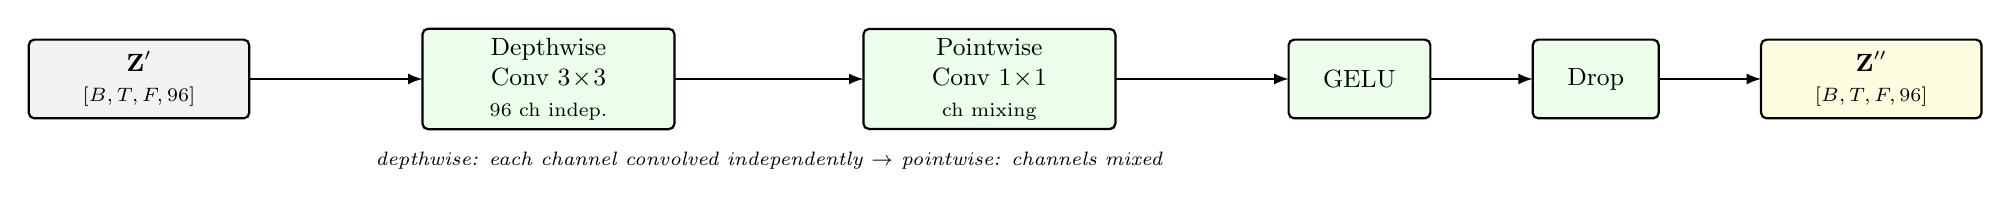
\begin{tikzpicture}[x=1cm, y=1cm, >=latex]
				\node[io, minimum width=2.8cm, minimum height=1.0cm] at (0.00,0.00) (zin) {$\mathbf{Z}'$\\{\scriptsize $[B,T,F,96]$}};
				\node[op, minimum width=3.2cm, minimum height=1.0cm] at (5.20,0.00) (dw) {Depthwise\\Conv $3\!\times\!3$\\{\scriptsize 96 ch indep.}};
				\node[op, minimum width=3.2cm, minimum height=1.0cm] at (10.80,0.00) (pw) {Pointwise\\Conv $1\!\times\!1$\\{\scriptsize ch mixing}};
				\node[op, minimum width=1.8cm, minimum height=1.0cm] at (15.50,0.00) (ge) {GELU};
				\node[op, minimum width=1.6cm, minimum height=1.0cm] at (18.50,0.00) (dr) {Drop};
				\node[outp, minimum width=2.8cm, minimum height=1.0cm] at (22.00,0.00) (zo) {$\mathbf{Z}''$\\{\scriptsize $[B,T,F,96]$}};
				\draw[thick, ->] (1.40,0.00) -- (3.60,0.00);
				\draw[thick, ->] (6.80,0.00) -- (9.20,0.00);
				\draw[thick, ->] (12.40,0.00) -- (14.60,0.00);
				\draw[thick, ->] (16.40,0.00) -- (17.70,0.00);
				\draw[thick, ->] (19.30,0.00) -- (20.60,0.00);
				\node[font=\scriptsize\itshape, anchor=north] at (8.00,-0.80) {depthwise: each channel convolved independently $\to$ pointwise: channels mixed};
			\end{tikzpicture}%
		}
		\caption{Section~4.7: Local depthwise-separable convolution.  Input $\mathbf{Z}'$ is the output of axial attention (Fig.~\ref{fig:sec46}).}
		\label{fig:sec47}
	\end{figure}
	
	\subsection{Feed-Forward MLP}
	
	\subsubsection*{Why another processing stage?}
	
	Attention (Section~4.6) captured long-range correlations across the grid.  The depthwise-separable convolution (Section~4.7) captured short-range local patterns.  But both of these operations are fundamentally about \emph{spatial} relationships---which positions should share information.  Neither one performs complex \emph{per-position} nonlinear computation.  The feed-forward MLP fills this gap: at each grid position independently, it takes the 96-dimensional feature vector and transforms it through a nonlinear function that can compute arbitrarily complex combinations of the features assembled by the preceding stages.
	
	\subsubsection*{What is FC (Fully Connected)?}
	
	``FC'' stands for \textbf{fully connected layer}, also called a \textbf{dense layer}---the simplest neural network operation.  It is exactly a matrix multiplication plus a bias vector:
	\begin{equation}
		\mathrm{FC}(\mathbf{x}) = W\,\mathbf{x} + \mathbf{b},
		\label{eq:fc}
	\end{equation}
	where $\mathbf{x} \in \mathbb{R}^{d_{\mathrm{in}}}$ is the input vector, $W \in \mathbb{R}^{d_{\mathrm{out}} \times d_{\mathrm{in}}}$ is a learned weight matrix, and $\mathbf{b} \in \mathbb{R}^{d_{\mathrm{out}}}$ is a learned bias.  The name ``fully connected'' comes from the fact that every output dimension depends on \emph{every} input dimension---row~$i$ of $W$ defines the $i$-th output as a weighted sum of all inputs.  This is the same operation as the $1\!\times\!1$ convolution in the stem (Section~4.3) and the pointwise convolution in Section~4.7---all three are matrix multiplications applied independently at each position.
	
	\subsubsection*{The expand-then-compress pattern}
	
	The MLP consists of two FC layers with a nonlinearity in between.  Follow the diagram (Fig.~\ref{fig:sec48}) left to right:
	
	\begin{enumerate}[nosep]
		\item \textbf{FC$_1$: $96 \to 192$ (expand).}  The 96-dimensional input vector is projected to 192 dimensions:
		\begin{equation}
			\mathbf{h}_{b,t,f} = W_1\,\mathbf{Z}''_{b,t,f,:} + \mathbf{b}_1, \qquad W_1 \in \mathbb{R}^{192 \times 96},\; \mathbf{b}_1 \in \mathbb{R}^{192}.
			\label{eq:mlp_fc1}
		\end{equation}
		This doubles the dimensionality, giving the network a wider intermediate space to work in.
		
		\item \textbf{GELU.}  The GELU nonlinearity is applied element-wise to the 192-dimensional vector.  Without this, the two FC layers would collapse into a single linear transformation $W_2 W_1 \mathbf{x} + (W_2 \mathbf{b}_1 + \mathbf{b}_2)$, which could be represented by one matrix---making the second layer redundant.  The nonlinearity between them is what gives the MLP its expressive power.
		
		\item \textbf{Dropout.}  Regularisation as described in Section~4.7.
		
		\item \textbf{FC$_2$: $192 \to 96$ (compress).}  The 192-dimensional vector is projected back to 96 dimensions:
		\begin{equation}
			\mathbf{Z}'''_{b,t,f,:} = W_2\,\Drop(\GELU(\mathbf{h}_{b,t,f})) + \mathbf{b}_2, \qquad W_2 \in \mathbb{R}^{96 \times 192},\; \mathbf{b}_2 \in \mathbb{R}^{96}.
			\label{eq:mlp_fc2}
		\end{equation}
		The output is back to 96 dimensions, matching the input size so it can be added back via the residual connection in the complete block (Section~4.9).
		
		\item \textbf{Dropout.}  A second dropout after the output projection.
	\end{enumerate}
	
	\subsubsection*{Why expand then compress?}
	
	The expansion ratio of~2 ($96 \to 192 \to 96$) creates a \textbf{bottleneck} architecture.  The intuition: the 96-dimensional input lives in a compressed representation.  By temporarily expanding to 192 dimensions, the network gains access to a richer space where it can form nonlinear combinations of features.  The GELU activation in this wider space can selectively activate or suppress different feature combinations.  The second FC layer then selects which of these 192 intermediate features are most useful and compresses them back to 96 dimensions for the next stage.
	
	An analogy: imagine you have 96 ingredients and want to cook a complex dish.  You first spread them out on a larger counter (192 slots) where you have room to combine them in various ways---mix some, heat others, leave some alone.  Then you plate the result back onto 96 slots, keeping only the useful combinations.
	
	\subsubsection*{``Applied independently at each grid position''}
	
	A critical point emphasised in the diagram: the \emph{same} weights $W_1, \mathbf{b}_1, W_2, \mathbf{b}_2$ are applied at every grid position $(t,f)$, but each position is processed \emph{independently}---position $(t\!=\!3, f\!=\!50)$ does not see position $(t\!=\!3, f\!=\!51)$ during this operation.  All spatial information exchange already happened in the attention and convolution stages; the MLP's job is purely per-position nonlinear transformation.
	
	\begin{keyidea}
		The four stages of each block have a clean division of labour.  Axial attention: long-range spatial information sharing.  Depthwise-separable convolution: short-range local patterns.  Feed-forward MLP: per-position nonlinear feature transformation.  Each stage does what the others cannot.
	\end{keyidea}
	
	
	
	\begin{figure}[ht!]
		\centering
		\resizebox{1.1\linewidth}{!}{%
			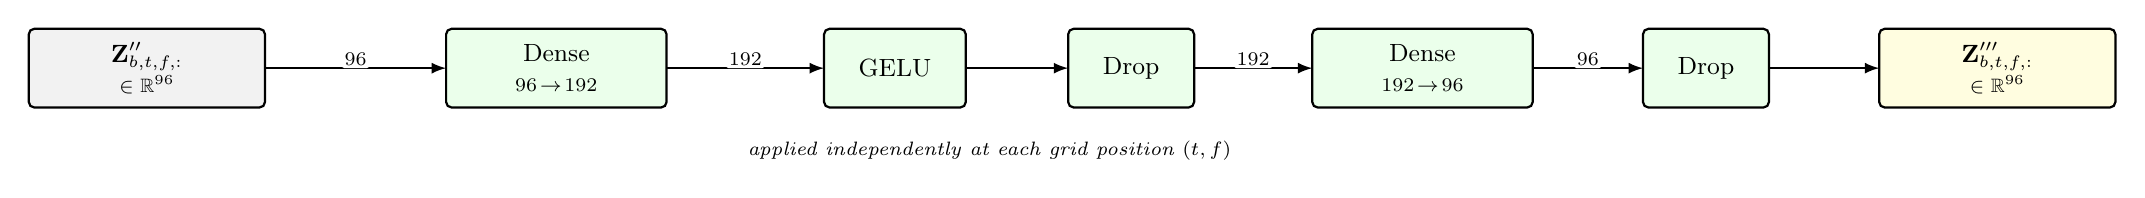
\begin{tikzpicture}[x=1cm, y=1cm, >=latex]
				\node[io, minimum width=3.0cm, minimum height=1.0cm] at (0.00,0.00) (zin) {$\mathbf{Z}''_{b,t,f,:}$\\{\scriptsize $\in\mathbb{R}^{96}$}};
				\node[op, minimum width=2.8cm, minimum height=1.0cm] at (5.20,0.00) (fc1) {Dense\\{\scriptsize $96\!\to\!192$}};
				\node[op, minimum width=1.8cm, minimum height=1.0cm] at (9.50,0.00) (ge) {GELU};
				\node[op, minimum width=1.6cm, minimum height=1.0cm] at (12.50,0.00) (d1) {Drop};
				\node[op, minimum width=2.8cm, minimum height=1.0cm] at (16.20,0.00) (fc2) {Dense\\{\scriptsize $192\!\to\!96$}};
				\node[op, minimum width=1.6cm, minimum height=1.0cm] at (19.80,0.00) (d2) {Drop};
				\node[outp, minimum width=3.0cm, minimum height=1.0cm] at (23.50,0.00) (zo) {$\mathbf{Z}'''_{b,t,f,:}$\\{\scriptsize $\in\mathbb{R}^{96}$}};
				\draw[thick, ->] (1.50,0.00) -- (3.80,0.00) node[lbl, pos=0.5, above] {96};
				\draw[thick, ->] (6.60,0.00) -- (8.60,0.00) node[lbl, pos=0.5, above] {192};
				\draw[thick, ->] (10.40,0.00) -- (11.70,0.00);
				\draw[thick, ->] (13.30,0.00) -- (14.80,0.00) node[lbl, pos=0.5, above] {192};
				\draw[thick, ->] (17.60,0.00) -- (19.00,0.00) node[lbl, pos=0.5, above] {96};
				\draw[thick, ->] (20.60,0.00) -- (22.00,0.00);
				\node[font=\scriptsize\itshape, anchor=north] at (10.70,-0.80) {applied independently at each grid position $(t,f)$};
			\end{tikzpicture}%
		}
		\caption{Section~4.8: Feed-forward MLP with expansion ratio 2.  Input $\mathbf{Z}''$ is the output of the local convolution (Fig.~\ref{fig:sec47}).}
		\label{fig:sec48}
	\end{figure}
	
	\subsection{The Complete Block}
	
	One FiLM axial refinement block combines all four stages---frequency attention, time attention, depthwise-separable convolution, and feed-forward MLP---with \textbf{pre-norm residual connections} (the dashed arrows in Fig.~\ref{fig:sec49}).  Understanding the skip connections is essential to understanding the diagram.
	
	\subsubsection*{What are skip connections (the dashed arrows)?}
	
	Look at Stage~1 in the diagram.  The input $\bZ^{(\ell)}$ flows along two parallel paths:
	\begin{itemize}[nosep]
		\item \textbf{The main path} (solid arrows): $\bZ^{(\ell)} \to \LN \to \FiLM \to \text{Freq MHA} \to \Drop$, producing some correction tensor.
		\item \textbf{The skip path} (dashed arrow): $\bZ^{(\ell)}$ goes directly to the $\oplus$ node, bypassing all processing.
	\end{itemize}
	The $\oplus$ node \emph{adds} the two together.  So the output of Stage~1 is:
	\begin{equation}
		\bZ^{(\ell,1)} = \underbrace{\bZ^{(\ell)}}_{\text{skip (identity)}} + \underbrace{\Drop\!\left(\MHA_f\!\left(\FiLM(\LN(\bZ^{(\ell)}), \bp)\right)\right)}_{\text{main path (learned correction)}}.
		\label{eq:skip1}
	\end{equation}
	The same pattern repeats for every stage: the stage's input is always added to the stage's output.  Each stage learns only a \textbf{correction} to its input, not the full representation from scratch.
	
	\subsubsection*{Why skip connections are essential}
	
	\textbf{1.\ Healthy gradient flow.}\quad During backpropagation, gradients must flow backward through every operation to update the weights.  Each operation (matrix multiply, nonlinearity, normalisation) slightly shrinks or distorts the gradient.  With $4$~blocks $\times$ $4$~stages~$= 16$ sequential operations, the gradient arriving at the first stage would be tiny---the early layers would barely learn.  The skip connections provide a \textbf{shortcut highway}: the gradient can flow directly through the $\oplus$ node and the dashed path, bypassing all the operations in between.  This keeps gradients healthy throughout the entire network.
	
	\textbf{2.\ Doing nothing is the default.}\quad Without skip connections, if a stage has nothing useful to contribute for a particular input, it would need to learn the identity function: output exactly what came in.  For a nonlinear multi-step pipeline ($\LN \to \FiLM \to \text{Conv} \to \GELU$), learning to perfectly reproduce the input is a non-trivial optimisation problem.  With the skip connection, doing nothing is the \textbf{default}---the stage just needs to output zeros, which is trivially easy.  This is the same principle as the global residual design (Section~3.2), where the output heads are zero-initialised so the network starts as the LS estimator.
	
	\textbf{3.\ Incremental refinement.}\quad Each stage builds on what the previous stages already achieved.  Stage~1 (freq attention) produces a useful representation.  Stage~2 (time attention) does not need to reconstruct it from scratch---it only adds what frequency attention missed.  Stage~3 (conv) adds local patterns that attention missed.  Stage~4 (MLP) adds per-position nonlinear refinements.  Each stage makes a small, targeted improvement.
	
	\begin{keyidea}
		Skip connections implement the same philosophy at every scale of the architecture.  At the \emph{global} level, the network learns a residual correction to the LS estimate ($\widehat{\bH}^{\mathrm{LS}} + 0.35\,\Delta\widehat{\bH}$).  At the \emph{block} level, each stage learns a residual correction to its input ($\bZ + \Delta\bZ$).  This ``learn the correction, not the full answer'' principle makes training stable, makes doing nothing easy, and enables incremental refinement.
	\end{keyidea}
	
	\subsubsection*{Reading the diagram: one full block}
	
	Follow the data flow through Fig.~\ref{fig:sec49} from $\bZ^{(\ell)}$ at the top-left to $\bZ^{(\ell+1)}$ at the bottom-right:
	
	\begin{enumerate}[nosep]
		\item \textbf{Stage~1 (freq attn):} $\bZ^{(\ell)}$ enters, is normalised (LN), conditioned on the prompt (FiLM), processed by frequency attention (Freq~MHA), regularised (Drop), and added to the skip.  Output: $\bZ^{(\ell,1)}$.
		
		\item \textbf{Stage~2 (time attn):} $\bZ^{(\ell,1)}$ follows the same pattern with time attention.  Output: $\bZ^{(\ell,2)}$.
		
		\item \textbf{Stage~3 (local conv):} $\bZ^{(\ell,2)}$ follows the same pattern with depthwise-separable convolution.  Output: $\bZ^{(\ell,3)}$.
		
		\item \textbf{Stage~4 (MLP):} $\bZ^{(\ell,3)}$ follows the same pattern with the feed-forward MLP.  Output: $\bZ^{(\ell+1)}$.
	\end{enumerate}
	
	The red arrows show the prompt $\bp_b$ entering every FiLM box from below---the \emph{same} prompt conditions all four stages (and all four blocks).
	
	\subsubsection*{The pre-norm pattern: LN before each stage}
	
	Notice that LayerNorm appears \emph{before} each stage's main operation, not after.  This is the ``pre-norm'' convention.  It normalises the features before they enter the attention or convolution, which stabilises training---especially in deeper networks.  The alternative (``post-norm'': normalise after the residual addition) is known to cause training instability in deep architectures.
	
	\subsubsection*{The equations}
	
	Letting $\bZ^{(\ell)}$ denote the input to block $\ell$, the four stages are:
	\begin{align}
		\bZ^{(\ell,1)} &= \bZ^{(\ell)} + \Drop\!\left(\MHA_f\!\left(\FiLM(\LN(\bZ^{(\ell)}), \bp)\right)\right), \\
		\bZ^{(\ell,2)} &= \bZ^{(\ell,1)} + \Drop\!\left(\MHA_t\!\left(\FiLM(\LN(\bZ^{(\ell,1)}), \bp)\right)\right), \\
		\bZ^{(\ell,3)} &= \bZ^{(\ell,2)} + \GELU\!\left(\PWConv\!\left(\DWConv\!\left(\FiLM(\LN(\bZ^{(\ell,2)}), \bp)\right)\right)\right), \\
		\bZ^{(\ell+1)} &= \bZ^{(\ell,3)} + \Drop\!\left(W_2\,\Drop\!\left(\GELU(W_1\,\FiLM(\LN(\bZ^{(\ell,3)}), \bp))\right)\right).
	\end{align}
	
	Every equation has the same structure: $\text{output} = \text{input} + f(\text{input})$, where $f$ is the stage's processing pipeline.  Read the ``$+$'' as the dashed skip connection in the diagram.
	
	The network uses $L = 4$ blocks, giving 16 total stages of processing.  The \emph{same prompt} $\bp$ modulates every stage in every block.
	
	
	
	\begin{figure}[ht!]
		\centering
		\resizebox{1.1\linewidth}{!}{%
			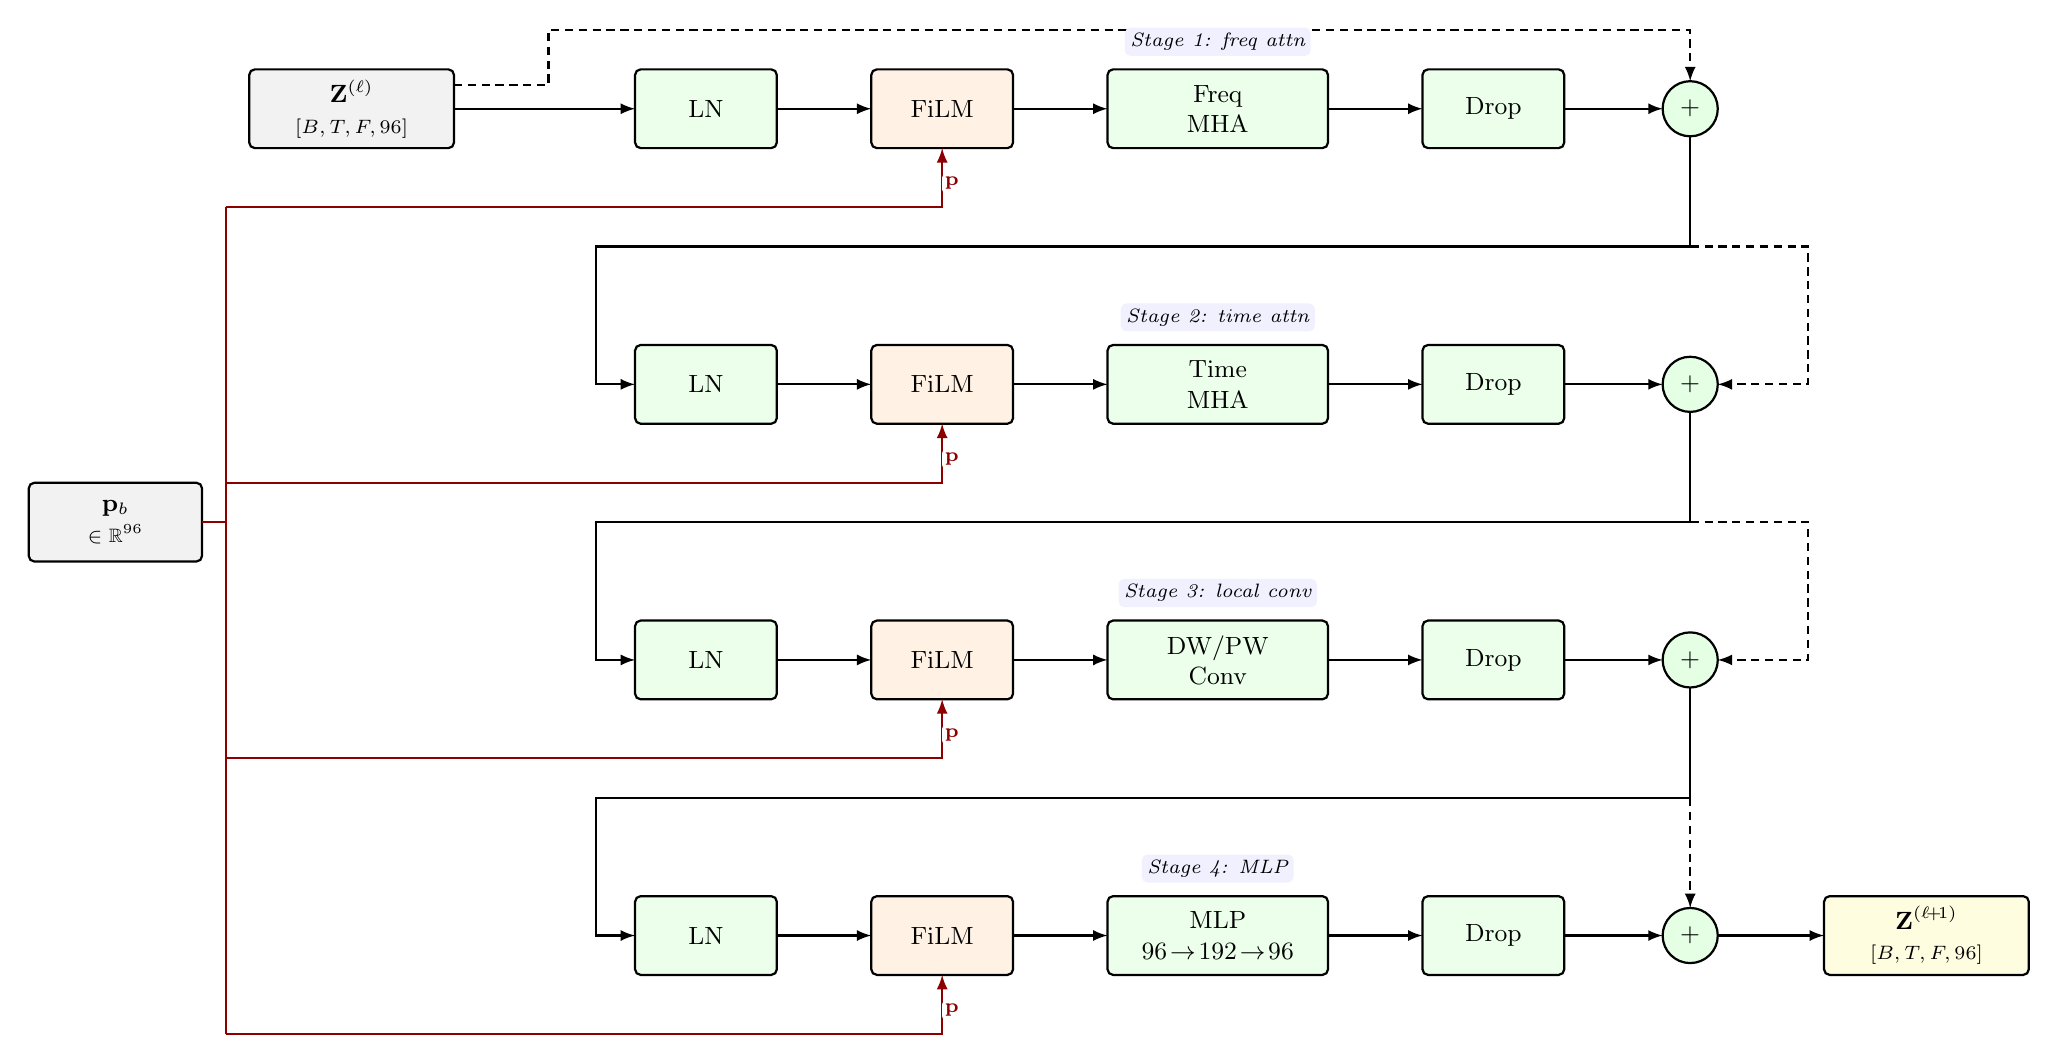
\begin{tikzpicture}[x=1cm, y=1cm, >=latex]
				\node[io, minimum width=2.6cm, minimum height=1.0cm] at (0.00,0.00) (zin) {$\mathbf{Z}^{(\ell)}$\\{\scriptsize $[B,T,F,96]$}};
				\node[op, minimum width=1.8cm, minimum height=1.0cm] at (4.50,0.00) (ln1) {LN};
				\node[aux, minimum width=1.8cm, minimum height=1.0cm] at (7.50,0.00) (fm1) {FiLM};
				\node[op, minimum width=2.8cm, minimum height=1.0cm] at (11.00,0.00) (s1) {Freq\\MHA};
				\node[op, minimum width=1.8cm, minimum height=1.0cm] at (14.50,0.00) (dr1) {Drop};
				\node[add, minimum width=0.7cm, minimum height=0.7cm] at (17.00,0.00) (a1) {$+$};
				\node[op, minimum width=1.8cm, minimum height=1.0cm] at (4.50,-3.50) (ln2) {LN};
				\node[aux, minimum width=1.8cm, minimum height=1.0cm] at (7.50,-3.50) (fm2) {FiLM};
				\node[op, minimum width=2.8cm, minimum height=1.0cm] at (11.00,-3.50) (s2) {Time\\MHA};
				\node[op, minimum width=1.8cm, minimum height=1.0cm] at (14.50,-3.50) (dr2) {Drop};
				\node[add, minimum width=0.7cm, minimum height=0.7cm] at (17.00,-3.50) (a2) {$+$};
				\node[op, minimum width=1.8cm, minimum height=1.0cm] at (4.50,-7.00) (ln3) {LN};
				\node[aux, minimum width=1.8cm, minimum height=1.0cm] at (7.50,-7.00) (fm3) {FiLM};
				\node[op, minimum width=2.8cm, minimum height=1.0cm] at (11.00,-7.00) (s3) {DW/PW\\Conv};
				\node[op, minimum width=1.8cm, minimum height=1.0cm] at (14.50,-7.00) (dr3) {Drop};
				\node[add, minimum width=0.7cm, minimum height=0.7cm] at (17.00,-7.00) (a3) {$+$};
				\node[op, minimum width=1.8cm, minimum height=1.0cm] at (4.50,-10.50) (ln4) {LN};
				\node[aux, minimum width=1.8cm, minimum height=1.0cm] at (7.50,-10.50) (fm4) {FiLM};
				\node[op, minimum width=2.8cm, minimum height=1.0cm] at (11.00,-10.50) (s4) {MLP\\$96\!\to\!192\!\to\!96$};
				\node[op, minimum width=1.8cm, minimum height=1.0cm] at (14.50,-10.50) (dr4) {Drop};
				\node[add, minimum width=0.7cm, minimum height=0.7cm] at (17.00,-10.50) (a4) {$+$};
				\node[outp, minimum width=2.6cm, minimum height=1.0cm] at (20.00,-10.50) (zout) {$\mathbf{Z}^{(\ell\!+\!1)}$\\{\scriptsize $[B,T,F,96]$}};
				\node[io, minimum width=2.2cm, minimum height=1.0cm] at (-3.00,-5.25) (pp) {$\mathbf{p}_b$\\{\scriptsize $\in\mathbb{R}^{96}$}};
				\draw[thick, ->] (1.30,0.00) -- (3.60,0.00);
				\draw[thick, ->] (5.40,0.00) -- (6.60,0.00);
				\draw[thick, ->] (8.40,0.00) -- (9.60,0.00);
				\draw[thick, ->] (12.40,0.00) -- (13.60,0.00);
				\draw[thick, ->] (15.40,0.00) -- (16.65,0.00);
				\draw[thick, ->, densely dashed] (1.30,0.30) -- (2.50,0.30) -- (2.50,1.00) -- (17.00,1.00) -- (17.00,0.35);
				\draw[thick, ->] (17.00,-0.35) -- (17.00,-1.75) -- (3.10,-1.75) -- (3.10,-3.50) -- (3.60,-3.50);
				\draw[thick, ->] (5.40,-3.50) -- (6.60,-3.50);
				\draw[thick, ->] (8.40,-3.50) -- (9.60,-3.50);
				\draw[thick, ->] (12.40,-3.50) -- (13.60,-3.50);
				\draw[thick, ->] (15.40,-3.50) -- (16.65,-3.50);
				\draw[thick, ->, densely dashed] (17.00,-0.35) -- (17.00,-1.75) -- (18.50,-1.75) -- (18.50,-3.50) -- (17.35,-3.50);
				\draw[thick, ->] (17.00,-3.85) -- (17.00,-5.25) -- (3.10,-5.25) -- (3.10,-7.00) -- (3.60,-7.00);
				\draw[thick, ->] (5.40,-7.00) -- (6.60,-7.00);
				\draw[thick, ->] (8.40,-7.00) -- (9.60,-7.00);
				\draw[thick, ->] (12.40,-7.00) -- (13.60,-7.00);
				\draw[thick, ->] (15.40,-7.00) -- (16.65,-7.00);
				\draw[thick, ->, densely dashed] (17.00,-3.85) -- (17.00,-5.25) -- (18.50,-5.25) -- (18.50,-7.00) -- (17.35,-7.00);
				\draw[thick, ->] (17.00,-7.35) -- (17.00,-8.75) -- (3.10,-8.75) -- (3.10,-10.50) -- (3.60,-10.50);
				\draw[thick, ->] (5.40,-10.50) -- (6.60,-10.50);
				\draw[thick, ->] (8.40,-10.50) -- (9.60,-10.50);
				\draw[thick, ->] (12.40,-10.50) -- (13.60,-10.50);
				\draw[thick, ->] (15.40,-10.50) -- (16.65,-10.50);
				\draw[thick, ->, densely dashed] (17.00,-7.35) -- (17.00,-10.15);
				\draw[thick, ->] (17.35,-10.50) -- (18.70,-10.50);
				% Vertical trunk from prompt node
				\draw[thick, red!55!black] (-1.90,-5.25) -- (-1.60,-5.25);
				\draw[thick, red!55!black] (-1.60,-1.25) -- (-1.60,-11.75);
				% Branch to FiLM 1: right then up into bottom
				\draw[thick, ->, red!55!black] (-1.60,-1.25) -- (7.50,-1.25) -- (7.50,-0.50) node[lbl, pos=0.4, right] {$\mathbf{p}$};
				% Branch to FiLM 2
				\draw[thick, ->, red!55!black] (-1.60,-4.75) -- (7.50,-4.75) -- (7.50,-4.00) node[lbl, pos=0.4, right] {$\mathbf{p}$};
				% Branch to FiLM 3
				\draw[thick, ->, red!55!black] (-1.60,-8.25) -- (7.50,-8.25) -- (7.50,-7.50) node[lbl, pos=0.4, right] {$\mathbf{p}$};
				% Branch to FiLM 4
				\draw[thick, ->, red!55!black] (-1.60,-11.75) -- (7.50,-11.75) -- (7.50,-11.00) node[lbl, pos=0.4, right] {$\mathbf{p}$};
				\node[font=\scriptsize\itshape, fill=blue!6, rounded corners=2pt, inner sep=2pt] at (11.00,0.85) {Stage 1: freq attn};
				\node[font=\scriptsize\itshape, fill=blue!6, rounded corners=2pt, inner sep=2pt] at (11.00,-2.65) {Stage 2: time attn};
				\node[font=\scriptsize\itshape, fill=blue!6, rounded corners=2pt, inner sep=2pt] at (11.00,-6.15) {Stage 3: local conv};
				\node[font=\scriptsize\itshape, fill=blue!6, rounded corners=2pt, inner sep=2pt] at (11.00,-9.65) {Stage 4: MLP};
			\end{tikzpicture}%
		}
		\caption{Section~4.9: One complete FiLM axial block.  Dashed = skip connections.}
		\label{fig:sec49}
	\end{figure}
	
	\subsection{Output Heads}
	
	After four blocks of processing, the network has a refined hidden tensor $\bZ^{(L)} \in \mathbb{R}^{B \times T \times F \times 96}$---a 96-dimensional feature vector at every grid position that encodes everything the network has learned about the channel.  But the downstream receiver does not need 96 abstract features; it needs two concrete physical quantities: a channel estimate and an error variance.  The output heads convert $\bZ^{(L)}$ into these two quantities through two parallel branches (top and bottom of Fig.~\ref{fig:sec410}).
	
	\subsubsection*{What are the $1 \times 1$ Conv2D blocks?}
	
	Both branches start with a $1 \times 1$ convolution---exactly the same operation as the stem (Section~4.3) and the pointwise convolution (Section~4.7): at each grid position independently, multiply the 96-dimensional vector by a learned weight matrix plus bias.  No spatial neighbours are involved; this is purely a \textbf{channel-dimension projection} that reduces from 96 internal features down to the number of physical output channels needed:
	
	\begin{itemize}[nosep]
		\item \textbf{Channel head:} $W_H \in \mathbb{R}^{4 \times 96}$, $\mathbf{b}_H \in \mathbb{R}^{4}$.  Output: 4 channels (real and imaginary parts for each of $N_r = 2$ receive antennas).  These are recombined into 2 complex-valued corrections $\Delta\widehat{H}_{b,t,f,r}$.
		\item \textbf{Variance head:} $W_V \in \mathbb{R}^{2 \times 96}$, $\mathbf{b}_V \in \mathbb{R}^{2}$.  Output: 2 channels (one per receive antenna).  These become the raw variance corrections $\Delta V_{b,t,f,r}$.
	\end{itemize}
	
	\subsubsection*{Branch~1: Channel correction (top of Fig.~\ref{fig:sec410})}
	
	Follow the top branch left to right:
	\begin{enumerate}[nosep]
		\item $\bZ^{(L)}$ enters the $1 \times 1$ Conv2D ($96 \to 4$, \textbf{zero-initialised}).
		\item The output is scaled by $\alpha_{\mathrm{res}} = 0.35$, producing $0.35\,\Delta\widehat{H}$.
		\item The $\oplus$ node adds the LS estimate $\widehat{H}^{\mathrm{LS}}$ (entering from above in the diagram).
	\end{enumerate}
	The final channel estimate is:
	\begin{equation}
		\widehat{H}^{\mathrm{UP}}_{b,t,f,r} = \widehat{H}^{\mathrm{LS}}_{b,t,f,r} + 0.35\,\Delta\widehat{H}_{b,t,f,r}.
		\label{eq:h_update}
	\end{equation}
	
	Because the Conv2D kernel and bias are both initialised to \textbf{zero}, before any training $\Delta\widehat{H} = 0$ everywhere, and the network outputs exactly the LS estimate.  The factor $0.35$ further dampens the correction during early training, preventing large random updates from destabilising the output.  Training can only improve upon the LS starting point.
	
	\subsubsection*{Branch~2: Error variance (bottom of Fig.~\ref{fig:sec410})}
	
	Follow the bottom branch:
	\begin{enumerate}[nosep]
		\item $\bZ^{(L)}$ enters a separate $1 \times 1$ Conv2D ($96 \to 2$, bias initialised to $-4.0$).
		\item The output passes through the \textbf{softplus} function.
		\item The $\oplus$ node adds the LS variance $V^{\mathrm{LS,bc}}$.
	\end{enumerate}
	The final variance estimate is:
	\begin{equation}
		\widehat{V}^{\mathrm{UP}}_{b,t,f,r} = V^{\mathrm{LS,bc}}_{b,t,f,r} + \softplus(\Delta V_{b,t,f,r}) + 10^{-6}.
		\label{eq:v_update}
	\end{equation}
	
	\subsubsection*{What is softplus and why use it?}
	
	Softplus is a smooth approximation to the ReLU function:
	\begin{equation}
		\softplus(x) = \ln(1 + e^x).
		\label{eq:softplus}
	\end{equation}
	Its key property: \textbf{the output is always positive}.  For large positive $x$, $\softplus(x) \approx x$.  For large negative $x$, $\softplus(x) \approx 0$.  Unlike ReLU, softplus never has a sharp corner and never outputs exactly zero, which gives smoother gradients during training.
	
	Variance is a physical quantity that \emph{must} be non-negative---a negative variance has no meaning.  If the network's raw output $\Delta V$ happens to be $-10$ (which can easily occur for a randomly initialised or early-training network), softplus maps it to $\softplus(-10) \approx 0.000045$, a small but positive number.  Without softplus, a raw negative output would produce a negative variance, which would cause numerical errors in the loss function and in the downstream detector.
	
	The bias initialisation of $-4.0$ means that before training, every position outputs $\softplus(-4.0) \approx 0.018$---a small positive value.  Combined with the LS variance anchor, this gives a reasonable starting point.
	
	\subsubsection*{Why predict error variance at all?}
	
	The channel correction head alone would indeed give you a better channel estimate than LS.  So why does the network also predict \emph{how uncertain} that estimate is at each grid position?
	
	\textbf{1.\ The downstream LMMSE detector needs it.}\quad After channel estimation, the receiver uses an LMMSE (Linear Minimum Mean-Square Error) equaliser to recover the transmitted data symbols.  The standard LMMSE formula is:
	\begin{equation}
		\widetilde{X}_{b,t,f} = \frac{\sum_{r} \widehat{H}^*_{b,t,f,r}\, Y_{b,t,f,r}}{\sum_{r} |\widehat{H}_{b,t,f,r}|^2 + \sigma^2_{\mathrm{eff}}},
	\end{equation}
	where $\sigma^2_{\mathrm{eff}}$ is the effective noise-plus-estimation-error power.  If the receiver uses only the thermal noise power $N_0$ for $\sigma^2_{\mathrm{eff}}$, it \textbf{overestimates the quality of its own channel estimate}---it trusts $\widehat{H}$ more than it should.  This causes the equaliser to amplify estimation errors instead of suppressing them.  By plugging in $\widehat{V}^{\mathrm{UP}}$ (which accounts for both noise \emph{and} residual estimation error), the detector makes better-calibrated soft decisions.
	
	\textbf{2.\ Position-dependent confidence.}\quad The error variance is predicted \emph{at every grid position independently}.  Pilot positions (where the network has direct observations) will typically have low predicted variance.  Data positions far from any pilot (where the network is extrapolating) will have higher predicted variance.  Positions in a deep fade (low SNR) will have higher variance than positions with a strong channel.  This \textbf{spatially varying confidence map} lets the downstream detector weight different positions appropriately---trusting the estimate more where it is reliable and being more cautious where it is not.
	
	\textbf{3.\ It improves training.}\quad The loss function (Section~5.1) contains a heteroscedastic NLL term:
	\[
	\mathcal{L}_{\mathrm{NLL}} = \mathrm{mean}\!\left(\frac{|E|^2}{\widehat{V}^{\mathrm{UP}} + \epsilon} + \log(\widehat{V}^{\mathrm{UP}} + \epsilon)\right),
	\]
	where $E = H - \widehat{H}^{\mathrm{UP}}$ is the estimation error.  The first term penalises large errors \emph{relative to the predicted variance}: if the network claims low variance but makes a large error, the penalty is severe.  The second term prevents the trivial solution of predicting infinite variance everywhere (which would make the first term zero).  Together, they force the network to learn a \emph{calibrated} uncertainty estimate---one that is honestly large where errors are large and honestly small where the estimate is accurate.
	
	\begin{keyidea}
		The channel head tells the receiver ``here is my best estimate of $H$.''  The variance head tells the receiver ``here is how much you should trust that estimate at each position.''  Without the variance head, the receiver treats every grid position with equal confidence, even though some positions are estimated much more accurately than others.  The variance map turns the channel estimate from a point prediction into a \textbf{calibrated probabilistic prediction}---and the downstream detector exploits this to make better decisions.
	\end{keyidea}
	
	% ========================================================================
	
	
	\begin{figure}[ht!]
		\centering
		\resizebox{1.1\linewidth}{!}{%
			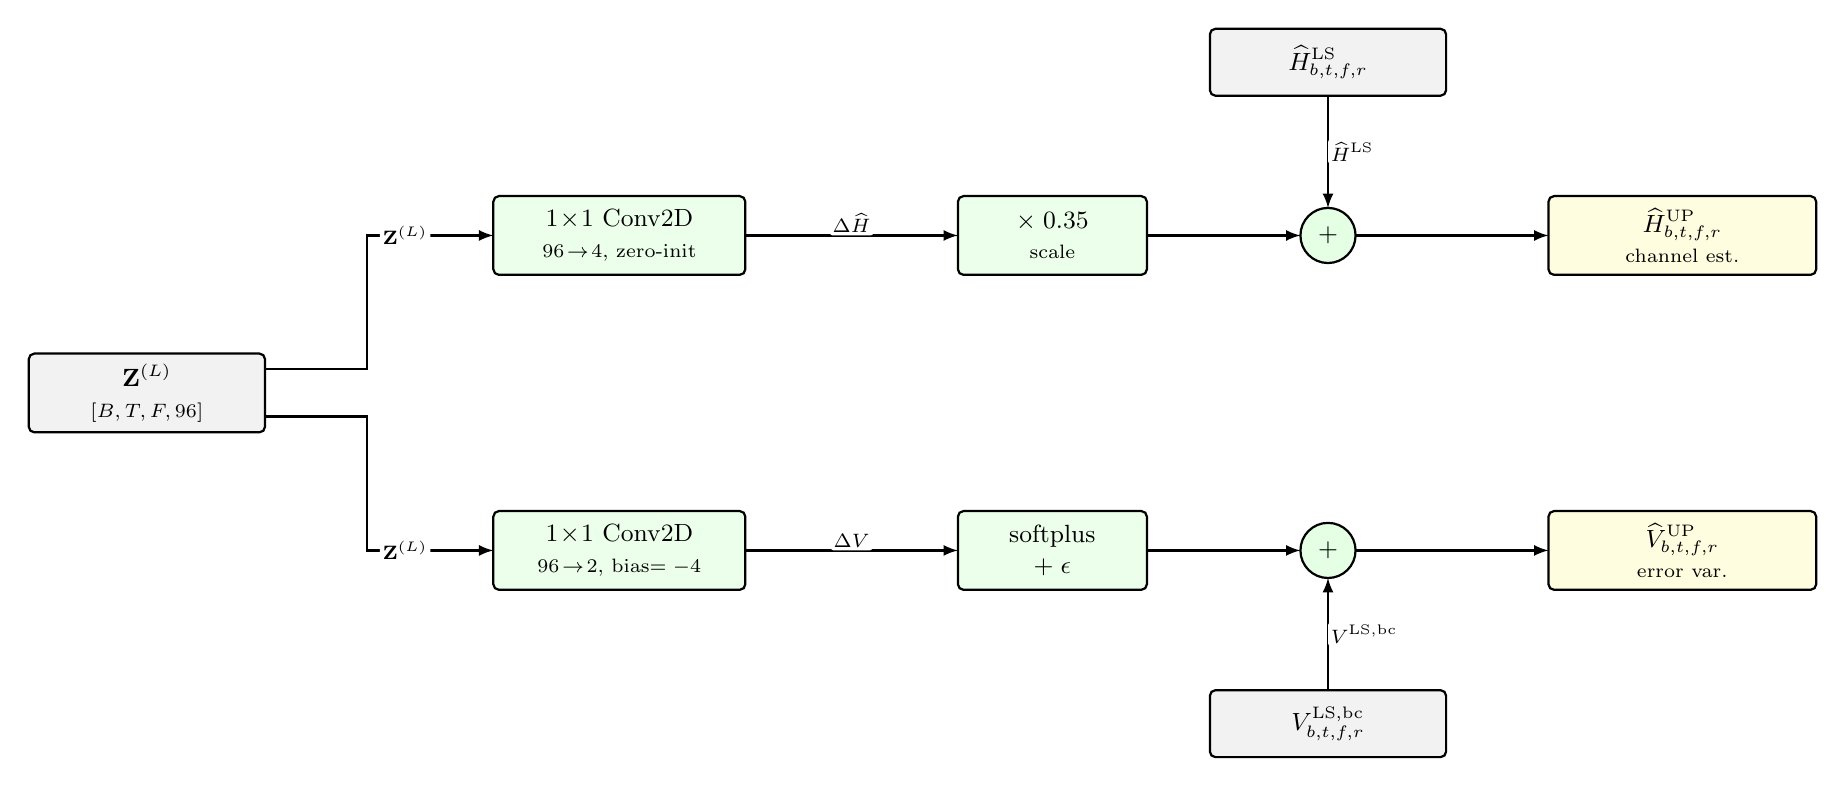
\begin{tikzpicture}[x=1cm, y=1cm, >=latex]
				\node[io, minimum width=3.0cm, minimum height=1.0cm] at (0.00,0.00) (zL) {$\mathbf{Z}^{(L)}$\\{\scriptsize $[B,T,F,96]$}};
				\node[op, minimum width=3.2cm, minimum height=1.0cm] at (6.00,2.00) (ch) {$1\!\times\!1$ Conv2D\\{\scriptsize $96\!\to\!4$, zero-init}};
				\node[op, minimum width=2.4cm, minimum height=1.0cm] at (11.50,2.00) (sc) {$\times\;0.35$\\{\scriptsize scale}};
				\node[add, minimum width=0.7cm, minimum height=0.7cm] at (15.00,2.00) (ah) {$+$};
				\node[outp, minimum width=3.4cm, minimum height=1.0cm] at (19.50,2.00) (ho) {$\widehat{H}^{\mathrm{UP}}_{b,t,f,r}$\\{\scriptsize channel est.}};
				\node[io, minimum width=3.0cm, minimum height=0.85cm] at (15.00,4.20) (hls) {$\widehat{H}^{\mathrm{LS}}_{b,t,f,r}$};
				\node[op, minimum width=3.2cm, minimum height=1.0cm] at (6.00,-2.00) (vh) {$1\!\times\!1$ Conv2D\\{\scriptsize $96\!\to\!2$, bias$=-4$}};
				\node[op, minimum width=2.4cm, minimum height=1.0cm] at (11.50,-2.00) (sp) {softplus\\$+\;\epsilon$};
				\node[add, minimum width=0.7cm, minimum height=0.7cm] at (15.00,-2.00) (av) {$+$};
				\node[outp, minimum width=3.4cm, minimum height=1.0cm] at (19.50,-2.00) (vo) {$\widehat{V}^{\mathrm{UP}}_{b,t,f,r}$\\{\scriptsize error var.}};
				\node[io, minimum width=3.0cm, minimum height=0.85cm] at (15.00,-4.20) (vls) {$V^{\mathrm{LS,bc}}_{b,t,f,r}$};
				\draw[thick, ->] (1.50,0.30) -- (2.80,0.30) -- (2.80,2.00) -- (4.40,2.00) node[lbl, pos=0.5, left] {$\mathbf{Z}^{(L)}$};
				\draw[thick, ->] (1.50,-0.30) -- (2.80,-0.30) -- (2.80,-2.00) -- (4.40,-2.00) node[lbl, pos=0.5, left] {$\mathbf{Z}^{(L)}$};
				\draw[thick, ->] (7.60,2.00) -- (10.30,2.00) node[lbl, pos=0.5, above] {$\Delta\widehat{H}$};
				\draw[thick, ->] (12.70,2.00) -- (14.65,2.00);
				\draw[thick, ->] (15.00,3.78) -- (15.00,2.35) node[lbl, pos=0.5, right] {$\widehat{H}^{\mathrm{LS}}$};
				\draw[thick, ->] (15.35,2.00) -- (17.80,2.00);
				\draw[thick, ->] (7.60,-2.00) -- (10.30,-2.00) node[lbl, pos=0.5, above] {$\Delta V$};
				\draw[thick, ->] (12.70,-2.00) -- (14.65,-2.00);
				\draw[thick, ->] (15.00,-3.78) -- (15.00,-2.35) node[lbl, pos=0.5, right] {$V^{\mathrm{LS,bc}}$};
				\draw[thick, ->] (15.35,-2.00) -- (17.80,-2.00);
			\end{tikzpicture}%
		}
		\caption{Section~4.10: Output heads.  Channel (top): zero-init residual $\times 0.35$ + LS.  Variance (bottom): softplus + LS variance.}
		\label{fig:sec410}
	\end{figure}
	
	\section{The Training Procedure}
	% ========================================================================
	
	\subsection{Loss Function}
	
	\subsubsection*{What is a loss function?}
	
	A loss function is the single number that tells the training algorithm ``how badly is the network performing on this batch of data?''  The optimiser (AdamW, in this case) adjusts all the network's weights to make this number smaller.  The choice of loss function determines \emph{what} the network learns to optimise: if you measure the wrong thing, the network will learn the wrong behaviour.
	
	UPAIR-5G's loss combines two terms with complementary roles.  Let $E_{b,r,t,f} = H_{b,r,t,f} - \widehat{H}^{\mathrm{UP}}_{b,r,t,f}$ be the estimation error---the difference between the true channel and the network's prediction:
	\begin{equation}
		\mathcal{L} = \underbrace{\mathrm{mean}\!\left(\frac{|E|^2}{\widehat{V}^{\mathrm{UP}} + \epsilon} + \log(\widehat{V}^{\mathrm{UP}} + \epsilon)\right)}_{\text{Heteroscedastic NLL}} + \underbrace{0.1 \cdot \frac{\mathrm{mean}(|E|^2)}{\mathrm{mean}(|\bH|^2) + \epsilon}}_{\text{Direct NMSE}}.
		\label{eq:loss}
	\end{equation}
	
	\subsubsection*{Term~1: Heteroscedastic NLL---what do these words mean?}
	
	This term has a strange-sounding name, but each word has a precise meaning:
	
	\textbf{NLL = Negative Log-Likelihood.}\quad This is a standard concept from probability.  The network's output defines a probability distribution over what the true channel $H$ might be: a Gaussian (normal distribution) centred at $\widehat{H}^{\mathrm{UP}}$ with variance $\widehat{V}^{\mathrm{UP}}$.  The \emph{likelihood} is the probability that this distribution assigns to the \emph{actual} true channel value $H$.  A good prediction assigns high probability to the truth (high likelihood); a bad prediction assigns low probability (low likelihood).  The \emph{negative log-likelihood} is $-\log(\text{likelihood})$: it turns ``higher is better'' into ``lower is better'' (which is what we need for a loss to minimise) and converts products into sums (which is numerically more stable).
	
	For a single Gaussian with mean $\mu$ and variance $\sigma^2$, the log-likelihood of observing value $x$ is:
	\begin{equation}
		\log p(x \mid \mu, \sigma^2) = -\frac{1}{2}\left(\frac{(x - \mu)^2}{\sigma^2} + \log \sigma^2\right) + \mathrm{const}.
		\label{eq:gaussian_nll}
	\end{equation}
	Dropping the constant and negating (since we minimise), the NLL to minimise is:
	\begin{equation}
		\frac{|E|^2}{\widehat{V}^{\mathrm{UP}}} + \log(\widehat{V}^{\mathrm{UP}}),
	\end{equation}
	which is exactly the first term of the loss (with $\epsilon$ added for numerical safety).
	
	\textbf{Heteroscedastic = position-dependent variance.}\quad The prefix ``hetero-'' means ``different,'' and ``scedastic'' relates to ``scatter'' or variance.  Heteroscedastic means the variance is \emph{different at different positions}.  This is the opposite of ``homoscedastic,'' where you would assume the same variance everywhere.  In UPAIR-5G, the network predicts a separate $\widehat{V}^{\mathrm{UP}}_{b,t,f,r}$ at every grid position, which is the heteroscedastic part.
	
	\subsubsection*{Why does the NLL have two sub-parts?}
	
	\textbf{Sub-part A:} $|E|^2 / \widehat{V}^{\mathrm{UP}}$ penalises large errors \emph{relative to the predicted variance}.  If the network claims low variance (``I am confident here'') but makes a large error, the ratio blows up and the penalty is severe.  If the network claims high variance (``I am uncertain here'') and makes a large error, the penalty is small---the network was honest about its uncertainty.
	
	\textbf{Sub-part B:} $\log(\widehat{V}^{\mathrm{UP}})$ prevents the trivial escape.  Without this term, the network could make sub-part~A zero by predicting $\widehat{V}^{\mathrm{UP}} \to \infty$ everywhere (``I am infinitely uncertain about everything'').  The log term penalises large variance, forcing the network to predict variance as \emph{small} as it honestly can.
	
	Together, the two sub-parts create a tension: predict variance too low and sub-part~A punishes you for overconfidence; predict variance too high and sub-part~B punishes you for being too cautious.  The optimum is a \textbf{calibrated} variance that honestly reflects the network's actual error at each position.
	
	\subsubsection*{Term~2: Direct NMSE}
	
	The second term is simpler:
	\begin{equation}
		\mathcal{L}_{\mathrm{NMSE}} = 0.1 \cdot \frac{\mathrm{mean}(|E|^2)}{\mathrm{mean}(|\bH|^2) + \epsilon}.
	\end{equation}
	
	This is the \textbf{Normalised Mean-Square Error}---the average squared estimation error divided by the average channel power.  Dividing by $|\bH|^2$ makes the metric scale-invariant: an error of $0.01$ on a channel of magnitude $1.0$ is treated the same as an error of $0.1$ on a channel of magnitude $10.0$.
	
	\emph{Why include it in addition to the NLL?}  Early in training, the variance prediction $\widehat{V}^{\mathrm{UP}}$ is poorly calibrated---the network has not yet learned what reasonable variance values look like.  The NLL term, which divides by $\widehat{V}^{\mathrm{UP}}$, can produce erratic gradient signals when the variance is poorly calibrated.  The NMSE term provides a \textbf{stable, direct gradient signal} that always points toward better channel estimates, regardless of the variance prediction's quality.  It acts as a stabiliser during early training.  The weight of $0.1$ keeps it secondary to the NLL once the variance prediction matures.
	
	\begin{keyidea}
		The two loss terms have complementary roles.  The NLL trains \emph{both} the channel estimate and the uncertainty map jointly, producing a calibrated probabilistic output.  The NMSE provides a stable gradient signal that ensures the channel estimate improves even when the variance prediction is still unreliable.  Together, they produce a network that outputs both an accurate channel estimate and an honest per-position confidence map.
	\end{keyidea}
	
	\subsection{Training Dynamics}
	
	\subsubsection*{Random $E_b/N_0$ sampling}
	
	Each training batch uses a uniformly random $E_b/N_0$ between $0$ and $18$\,dB.  This is essential: the network must work across a wide range of SNR conditions, not just one.  If trained at a fixed SNR, the network would overfit to that noise level.  Random sampling forces the network (and its prompt) to handle everything from very noisy ($0$\,dB) to relatively clean ($18$\,dB) channels.  This is also why the prompt mechanism (Section~4.4) is so important---it lets the same weights adapt their behaviour based on the current slot's SNR.
	
	\subsubsection*{AdamW optimiser}
	
	AdamW is a variant of the Adam optimiser that properly decouples weight decay from the adaptive learning rate.  The key hyperparameters:
	\begin{itemize}[nosep]
		\item \textbf{Learning rate $3 \times 10^{-4}$}: How large a step to take in each weight update.
		\item \textbf{Weight decay $10^{-5}$}: A small penalty that shrinks weights toward zero each step, preventing any single weight from growing too large (regularisation).
		\item \textbf{Gradient clipping at global norm $1.0$}: If the total gradient magnitude exceeds $1.0$, all gradients are rescaled down.  This prevents rare ``exploding gradient'' events (e.g., from an unusual batch) from destabilising the network.
	\end{itemize}
	
	\subsubsection*{Training schedule}
	
	\begin{itemize}[nosep]
		\item \textbf{5000 training steps,} batch size 48.  Each step processes 48 independent slot realisations.
		\item \textbf{Validation every 250 steps} at $E_b/N_0 = 7$\,dB (the middle of the evaluation grid), using 96 batches.  This monitors whether the network is improving or starting to overfit.
		\item \textbf{Best checkpoint} saved by validation NMSE.  The final deployed model is not the one from the last training step (which might have overfit), but the one that performed best on the held-out validation set.
	\end{itemize}
	
	% ========================================================================
	\section{The Phase-Aware Configured Reservoir Baseline}
	% ========================================================================
	
	This is the most sophisticated classical baseline.  It uses no gradient training, only offline covariance statistics and a per-slot linear solve.
	
	\subsection{Covariance Estimation}
	
	The implementation generates channel samples (with $N_0 = 0$), converts each to $[B, T, F, N_r]$, and computes empirical time, frequency, and spatial covariances by accumulating row-Gram matrices.  These are Hermitianized and diagonally loaded.
	
	\subsection{Basis Construction}
	
	\textbf{Time basis:} Top-$K_t = 6$ eigenvectors of $\bR_t$ plus 5 deterministic phase-slope modes $u_m^{\mathrm{phase}}[t] = e^{j\rho_m(t - t_{\mathrm{DMRS}})}$ with $\rho_m \in \{-0.12, -0.06, 0, 0.06, 0.12\}$\,rad.
	
	\textbf{Frequency basis:} Top-$K_f = 10$ eigenvectors of $\bR_f$ plus 4 DCT modes $u_k^{\mathrm{dct}}[f] = \cos\!\left(\frac{\pi(f+\frac{1}{2})k}{F}\right)$.
	
	The full design matrix is the Kronecker product:
	\begin{equation}
		\bPhi = \bU_t \otimes \bU_f^*.
	\end{equation}
	
	\subsection{Per-Slot Solve}
	
	The phase-aware version first applies DD-CPE as a preconditioner, extracts a per-symbol phasor, and de-rotates the LS estimate to a phase-normalised work domain.  It then solves a regularised weighted linear system at pilot positions:
	\begin{equation}
		\widehat{\bc}_{b,r} = \left(w_{b,r}\, \bPhi_\mathcal{P}^H \bPhi_\mathcal{P} + \bLambda^{-1} + \tau\bI\right)^{-1} w_{b,r}\, \bPhi_\mathcal{P}^H\, \bh^{\mathrm{work,pilot}}_{b,r},
	\end{equation}
	reconstructs the full grid $\widehat{\bh} = \bPhi\,\widehat{\bc}$, limits residual power, re-rotates to the original domain, and blends with the DD-CPE anchor using $\lambda_{\mathrm{LS}} = 0.55$.
	
	% ========================================================================
	\section{Evaluation Methodology}
	% ========================================================================
	
	\subsection{Adaptive Monte Carlo}
	
	For each \EbNo{} point, at least 256 batches are processed.  Evaluation continues until all stopping receivers accumulate 100 block errors, or 1024 batches are reached.  This ensures reliable BER/BLER estimates without wasting compute at operating points where errors are frequent.
	
	\subsection{Reliability Flags}
	
	A BER point is marked ``reliable'' if at least 100 bit errors were observed.  A BLER point requires at least 20 block errors.  These flags control which points appear in the publication plots.
	
	\subsection{Metrics}
	
	\begin{align}
		\text{BER} &= \frac{\text{bit\_errors}}{\text{num\_bits}}, \\
		\text{BLER} &= \frac{\text{block\_errors}}{\text{num\_blocks}}, \\
		\text{NMSE} &= \frac{1}{N_{\mathrm{batches}}} \sum_i \frac{\|\bH_i - \widehat{\bH}_i\|^2}{\|\bH_i\|^2}.
	\end{align}
	
	All receivers process the same batches with the same channel realisations, phase impairments, and noise.
	
	\subsection{Three Scenarios}
	
	\begin{center}
		\begin{tabular}{lcc}
			\toprule
			Scenario & Phase impairment & DMRS positions \\
			\midrule
			Mild main & Enabled & 1 (standard) \\
			Mild clean & Disabled & 1 (standard) \\
			Mild DMRS-rich & Enabled & 2 (additional) \\
			\bottomrule
		\end{tabular}
	\end{center}
	
	The clean scenario isolates the learned front-end's value from phase tracking.  The DMRS-rich scenario tests whether the advantage disappears with richer pilot support (it shrinks in BER/BLER but grows in NMSE).
	
	% ========================================================================
	\section{Why UPAIR-5G Works: The Complete Picture}
	% ========================================================================
	
	\subsection{The Information Advantage}
	
	Classical estimators use pilot observations and a statistical model.  UPAIR-5G adds the \textbf{raw received signal at data positions}.
	
	At a data position, $Y = H \cdot X + N$.  The receiver doesn't know $X$, but $X$ is from a 64-QAM constellation (one of 64 discrete points).  So $Y$ is not arbitrary: it's constrained to lie near one of 64 scaled-and-rotated versions of $H$.  The network learns to exploit this structure to refine its channel estimate---similar in spirit to DD-CPE, but without committing to hard decisions.
	
	\subsection{The Prompt as Automatic Mode Selection}
	
	Different slots have different characteristics.  Classical estimators use fixed algorithms; DD-CPE has fixed hyperparameters.  UPAIR-5G's prompt automatically calibrates the network's behaviour: strong/stable pilots produce confident modulation, noisy/unstable pilots produce conservative modulation.
	
	\subsection{Residual Learning as a Structural Prior}
	
	The zero-initialised residual design means the network starts from a physics-based anchor (LS) and can only improve it.  Early in training, the corrections are small and the loss landscape is smooth.  This avoids the challenging optimisation that would arise from predicting the full channel from scratch.
	
	\subsection{Measured Results}
	
	In the mild-main scenario, UPAIR-5G achieves:
	\begin{itemize}[nosep]
		\item \textbf{3--5$\times$ lower NMSE} than the best classical receiver (average ratio: exactly 4.00$\times$).
		\item \textbf{Up to 17$\times$ lower BER} at 8\,dB \EbNo{}.
		\item \textbf{Up to 17$\times$ lower BLER} at the same operating point.
	\end{itemize}
	
	The gain persists in all three scenarios.  In the clean scenario (no phase impairment), the NMSE advantage ranges from 3.65$\times$ to 5.20$\times$, confirming the gain is not solely from phase tracking.
	
	% ========================================================================
	\section{Summary}
	% ========================================================================
	
	UPAIR-5G is a drop-in replacement for the channel estimation front end in a 5G~NR PUSCH receiver.  It takes the standard LS channel estimate as a starting point, augments it with the raw received signal, noise level, and pilot mask as additional features, lifts these into a learned representation, conditions that representation on a per-slot prompt extracted from pilot positions, refines it through four blocks of FiLM-modulated axial attention and local convolution, and outputs a residual channel correction and a calibrated error-variance map.  The downstream LMMSE detector and LDPC decoder are unchanged.  The entire advantage comes from a single forward pass with fixed weights---no gradient descent at inference, no cross-slot state, no extra information beyond what any classical receiver already has access to.
	
\end{document}